\chapter{Properties of Neutrino Emission}
\label{chap:ray_tracing}

The leakage approximation used in Chap.~\ref{chap:leakage} gives us a beginning
understanding of the cooling effects of neutrinos on the accretion disk, or
how the disk changes as it radiates. Through that approximation we have been able
to estimate changes in the energy and composition of the fluid at the position
$x^\alpha$ due to the emission of neutrinos at $x^\alpha$.

However, the leakage approximation teaches us very little about the properties of
that emission. We \emph{can} extract some rough global measures:
1) the sum of the energy losses from all positions in the disk (i.e.\
the volume integral of $Q_{\nu_i}$ defined in Sec.~\ref{sec:leakage})
gives us the total energy luminosity, $L_{\nu_i}$, at any epoch,
2) likewise the sum of $R_{\nu_i}$ gives us the total lepton number luminosity
(also denoted $R_{\nu_i}$),
3) and the ratio of these two luminosities gives us the average neutrino energy,
$\langle \varepsilon_{\nu_i} \rangle$. These three calculations are presented in
Fig.~\ref{fig:neutrinos_by_species}.

But to answer some of the questions presented in Chap.~\ref{chap:overview}, we
need to know more about the radiation field outside of the disk, particularly
how it varies with position, $x^\alpha$, and how it is distributed in energy and
angle, $p_k$.
That is, we need to develop an estimate of the neutrino distribution function,
$f_{\nu_i}(x^\alpha;p_k)$.

Where the mean free path of the neutrinos is long with respect to local fluid
\todo{show this is the case}
scales at $x^\alpha$, $f_\nu(x^\alpha)$ is dependent upon the state of matter
far away from $x^\alpha$. In lieue of solving the Boltzmann equation in full
\todo{ref eqn in Chap.~\ref{chap:intro}}
(which would involve an evolution of a scalar field like those presented in
Chap.~\ref{chap:leakage} for fluid and metric fields, but over a 6-dimensional
phase space manifold with coordinates $\{x^j,p_k\}$, and therefore
computationally out of reach today),
we can capture this nonlocality with a ray tracing solution.
In ray tracing, $f_\nu(x^\alpha;p_k)$ is computed by tracing a neutrino trajectory
backwards from $x^\alpha$ with a momentum $p_k$, keeping track of additions
and depletions to the neutrino number density along that trajectory.
Each ray yields an approximate solution to the Boltzmann equation at a
single point on the phase space manifold of interest. A ray
tracing solution to the Boltzmann equation places an observer at $x^\alpha$,
points him in the direction $p_k$, and asks ``how many neutrinos from that
direction?''
This approximation neglects additions to the neutrino number density due to
scattering into the line of sight (the kind of scattering that gives to the
moon or a streetlamp a halo on a foggy night).
\todo{ref later discussion}

In this chapter I present a ray tracing algorithm for estimating
$f_{\nu_i}(x^\alpha;p_k)$ in relativistic numerical spacetimes and fluid
distributions, I calculate $f_{\nu_i}$ describing neutrino
emission from the model accretion disk from Chap.~\ref{chap:leakage},
and I use these $f_\nu$s to estimate $q_{\nu\bar{\nu}}$, the heating due to
neutrino-antineutrino annihilation in the funnel of the disk.
Because of large uncertainties,
this last calculation should be considered a proof-of-concept for future
calculations. It may also be considered a back-of-the-envelope answer to
the question, ``Can a neutron star--black hole merger drive a gamma ray burst
jet by neutrino processes alone?''

Sec.~\ref{sec:f_algorithm} gives a technical overview of the ray tracing
algorithm and two code tests. Sec.~\ref{sec:f_this_case} presents the distribution
function of the three 'leakage' neutrino species around this model accretion
disk. Secs.~\ref{sec:q_algorithm}~and~\ref{sec:q_this_case} describe the
algorithm for and results from a neutrino-antineutrino annihilation heating
calculation for this model.

\section{Calculating $f_\nu$}
\label{sec:f_algorithm}

In the most comprehensive treatment, a ray tracing solution for $f_\nu$ is calculated
by solving the rendering equation backwards along a trajectory terminating at
$x^a$ with momentum $p_k$:
\todo{derive rendering eqn, or check/ref below}
\begin{equation}
  \label{eqn:rendering}
  f(x^\alpha;p_k) = \int_{x^a}^{\rm far\,away} \diff \lambda \, \mathcal{E}(p_k)
  \exp\left(-\int_{x^a}^\lambda  \diff \lambda' \, \mathcal{A}(p_k)\right)
\end{equation}
where $\mathcal{E}$ and $\mathcal{A}$ are the invariant emissivity and opacity
defined in Chap.~\ref{chap:intro}.
\todo{ref eqns}
For isotropic scattering, $p_k$ only enters $\mathcal{E}$ and $\mathcal{A}$ in the
form $-p_\beta u^\beta$, the neutrino energy in the rest frame of the fluid.
Furthermore, $p_\beta$ may be calculated from $p_i$ by invoking the neutrino mass,
$-m_{\nu_i}^2=p_\beta p^\beta$.
All the neutrino masses are vanishingly small in the case of nuclear
accretion disks, with fluid energy scales of a few MeV. So in the following we
set $m_{\nu_i}=0$.

As $f_\nu$ accumulates along the ray, the integrand in Eqn.~\ref{eqn:rendering}
gets attenuated by the exponential term, which is the optical depth defined in
Chap.~\ref{chap:intro}.
\todo{ref eqn}
At large optical depths, the integrand vanishes exponentially, because fluid
properties on the far side of opaque matter cannot affect the neutrino
distribution function on this side. The exponential behavior of the integrand
leads us to pose a further approximation, that all neutrinos are emitted from
a single point along the trajectory, the neutrinosurface.

In this treatment, the ray is traced backwards until the optical depth becomes
large ($\tau\sim1$). This defines the neutrinosurface at $x_0^\alpha$. The
neutrinos are assumed to decouple from the matter at this surface, and so f
is simply the Fermi-Dirac distribution:
\begin{equation}
  \label{eqn:f_fermi_dirac}
  f(x^\alpha;p_k) =
  \left(\exp\left(\frac{-p_\beta u^\beta(x_0^\alpha)}{T(x_0^\alpha)}
  -\eta(x_0^\alpha) \right)+1\right)^{-1}
\end{equation}
where $T(x_0^\alpha)$ is the fluid temperature at the neutrinosurface, and
$\eta(x_0^\alpha)$ is the neutrino chemical potential scaled by $T$.
We use $\eta$ estimated by the leakage scheme (Eqn.~\ref{mu_nu}).
\todo{other choices for $\eta$}

Because neutrino scattering processes scale with
$\varepsilon^2=(-p_{\nu}^\beta u^\beta)^2$,
\todo{ref intro}
we use the energy-factored opacity $\zeta=\chi/\varepsilon^2$, where $\chi$ is
the cumulative opacity:
\begin{equation}
  \chi = \sum\limits_{{\rm processes}\, i} \chi_i.
\end{equation}
We consider scattering by nucleons and nuclei and absorption onto nucleons,
as described in Sec.~\ref{sec:leakage}.
Because the fluid and spacetime configuration at this late time is approximately
axisymmetric and stationary on the timescale of a neutrino-crossing time
($\sym1$~ms), we trace our geodesics through a single time slice of data,
rather than taking timesteps backwards through previous data slices,
interpolating in between slices. This greatly reduces the memory demands (each
time slice comprises $\sym$1~GB of data) and complexity of the calculation.
\todo{estimate disk changes over 1~ms: from response to leakage referee}

\subsection{Geodesic and Opacity Equations}
\label{ssec:geodesic}
In a general spacetime like that of our disk model, neutrinos do not follow
straight Euclidean paths, but curves that obey the geodesic equation,
\begin{equation}
  \label{eqn:geodesic}
  0=\frac{d^2x^\alpha}{d\lambda^2} + \Gamma^\beta_{\alpha\gamma}
  \frac{dx^\alpha}{d\lambda}\frac{dx^\gamma}{d\lambda},
\end{equation}
This second-order equation may be split into two coupled first-order equations
by choosing the affine parameterization $\lambda$ such that
$dx^\alpha/d\lambda=p^\alpha$ and
$dp^\beta/d\lambda=\Gamma^\beta_{\alpha\gamma}p^\alpha p^\gamma$.
\todo{umm, check p eqn}
The connection coefficients may be calculated from derivatives of the metric,
\begin{eqnarray}
  \label{eqn:christoffel}
  \Gamma^\beta_{\alpha\gamma}
  &=& \psi^{\beta\mu}\Gamma_{\mu\alpha\gamma} \nonumber \\
  &=& \frac{1}{2} \psi^{\beta\mu}
  (\psi_{\mu\alpha,\gamma} + \psi_{\mu\gamma,\alpha} - \psi_{\alpha\gamma,\mu}).
\end{eqnarray}

Neutrinos have rest masses less than a few eV \citep{oliv2014-pdg}.
Therefore, at the neutrino energy scale
of this problem (a few MeV, see Fig.~\ref{fig:neutrinos_by_species}), the
geodesics are essentially null.
\todo{say why this matters}

We integrate the geodesic equations parameterized by coordinate time,
using the formulation introduced by \cite{hugh1994-eh_finding}.
The extensive framework to integrate the \citeauthor{hugh1994-eh_finding}\
equations through a numerical spacetime demands efficient handling of
pointwise interpolation of metric fields to arbitrary positions, reading from
disk and reconstructing into memory the metric data dumped from a previous
simulation, and accurate integration of a system of ordinary differential
equations.
All of this was implemented by a graduate student at Cornell, Andy Bohn, in order
to find event horizons and compute gravitational lensing; the latter was
published in \cite{bohn2015-lensing}.
I piggy backed my ray tracing code on top of his general and efficient framework.

In addition to equations for $x^j$ and $p_k$, we integrate $\tau$, the optical
depth along the ray. Thus our entire system of equations is
\begin{eqnarray}
  \label{eqn:geo_x}
  \frac{dx^j}{dt} &=& g^{ji}\frac{p_i}{p^t} - \beta^j \\
  \label{eqn:geo_p}
  \frac{dp_k}{dt} &=& -\alpha \alpha_{,k}p^t + \beta^i_{,k}p_i
  - \frac{1}{2}g^{ji}_{,k} \frac{p_jp_i}{p^t} \\
  \label{eqn:geo_tau}
  \frac{d\tau}{dt} &=& \frac{\varepsilon^3}{p^t} \zeta,
\end{eqnarray}
where $\alpha$ is the lapse, $\beta^j$ the shift, $g^{ij}$ the inverse
induced metric on the spatial slice, and $\varepsilon$ is the neutrino
energy in the frame comoving with the fluid.

A word on $p^t$, used in Eqns.~\ref{eqn:geo_x}--\ref{eqn:geo_tau}.
As is well-known, $p_t$ does not change along a geodesic trajectory if the
spacetime is stationary. (This result may be derived directly from the geodesic
equation, Eqn.~\ref{eqn:geodesic}.)
However, $p^t$, in general, \emph{does} change. We may calculate it in the
following steps: 1) enforce $p_\alpha p^\alpha=0$ by calculating
$p_t=p_i\beta^i-\alpha\sqrt{p_ip_jg^{ij}}$, so that all four components of the
momentum 1-form are known, then 2) calculate the time-component of the dual of
this 1-form, $p^t=\psi^{t\alpha}p_\alpha$, where $\psi^{\alpha\beta}$ may be
computed from the lapse, shift, and induced spatial metric by matrix inversion.

A word on $\varepsilon=-p_\alpha u^\alpha$, used in Eqn.~\ref{eqn:geo_tau}.
In our simulations we don't store $u^\alpha$ directly, but rather the spatial
components of the fluid four-velocity 1-form, $u_i$, and the fluid Lorentz
factor, $W$. (The Lorentz factor doesn't need to be stored, since it may
be calculated from the normalization of $u^\alpha$, by
$W=(u_iu_jg^{ij}+1)^{1/2}$. However it is used throughout our code in enough
places that storing $W$ improves our code's efficiency.)
From these variables, we may calculate
\begin{equation}
  \varepsilon = -p_t W/\alpha -p_i(u_j g^{ij}-\beta^i W/\alpha).
\end{equation}

\subsection{Momentum Conventions}
\label{ssec:p_conventions}
Because of the natural symmetries of our spacetime, it is more convenient to use
momentum components in spherical polar than in cartesian representation. We
describe the map between these representations here.

The neutrino's 4-momentum is fully specified by three numbers, the fourth being
constrained by the mass of the neutrino, which vanishes with respect to the
energies in this problem. Instead of using three of the spherical polar
components, we define a Euclidean magnitude, $p$, and two angles $\alpha$,
$\beta$ which map to the cartesian components of the covariant 4-momentum by
the standard spherical polar map
\begin{align}
  &p_x = p\sin\alpha\cos\beta \\
  &p_y = p\sin\alpha\sin\beta \\
  &p_z = p\cos\alpha,
\end{align}
so that $p = (p_x^2+p_y^2+p_z^2)^{1/2}$.
Fig.~\ref{fig:p_conventions} provides a visual reference for these definitions.

\begin{figure}
  \centering
  \begin{subfigure}{.5\textwidth}
    \centering
    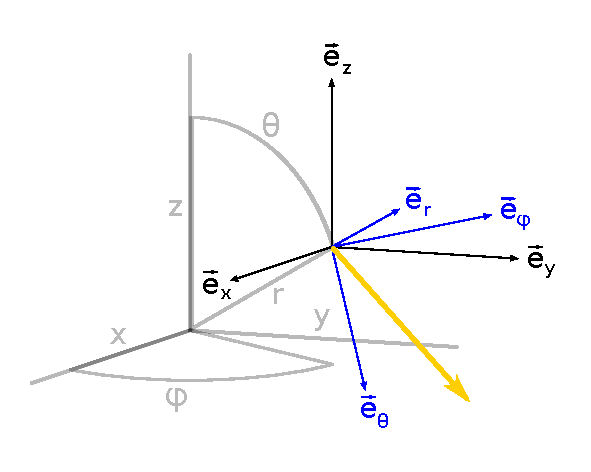
\includegraphics[width=1\linewidth]{Figures/spherical_polar_map}
  \end{subfigure}
  \begin{subfigure}{.45\textwidth}
    \centering
    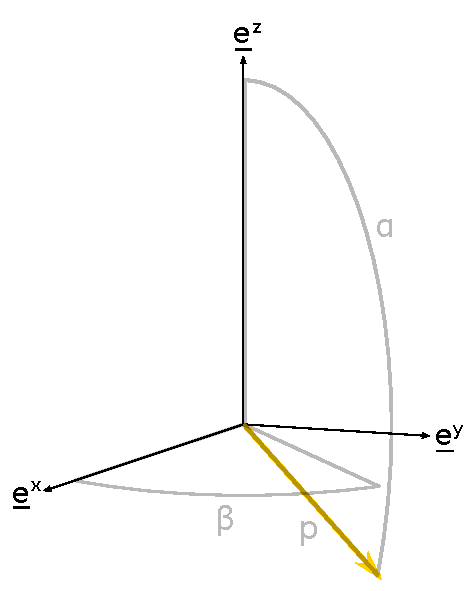
\includegraphics[width=0.8\linewidth]{Figures/neutrino_momentum_conventions}
  \end{subfigure}
  \caption[Conventions for momentum components]{
    In both diagrams, the broad yellow arrow represents the neutrino's momentum.
    \emph{Left Figure}:
    Spatial basis vectors ($\vec{e}_i\equiv\partial/\partial x^i$)
    at a representative position on the manifold.
    The coordinates $\{r,\theta,\phi\}$ are defined with respect to
    $\{x,y,z\}$ by the standard spherical polar to cartesian map
    (e.g.\ $x=r\sin\theta\cos\phi$).
    The spherical basis vectors are blue, and the cartesian basis vectors black.
    \emph{Right Figure}:
    The cotangent space at the neutrino's position.
    The neutrino momentum 1-form, $p_\mu$,
    may be written componentwise using the basis dual to $\vec{e}_i$
    ($\underline{e}^i\equiv dx^i$).
    The neutrino momentum is completely specified by three numbers.
    We use $\{p_t$,$\alpha$,$\beta\}$, which describe the cartesian spatial
    components of $p_\mu$ with the standard spherical polar to cartesian map
    (e.g.\ $p_x=p\sin\alpha\cos\beta$).
    The $p$ in these formulae is the Euclidean magnitude,
    $p = (p_x^2+p_y^2+p_z^2)^{1/2}$, related to $p_t$ by
    Eqns.~\ref{eqn:p_to_pt}~and~\ref{eqn:angular_factor}.
    (Note, we draw the neutrino's momentum vector embedded in the
    spatial manifold in the left figure, even though it properly lives only in
    the cotangent space in the right figure.)
    }
  \label{fig:p_conventions}
\end{figure}

To clean up some future calculations, we also define a 1-form on the
spatial manifold, $\Omega_i$, so that
\begin{align}
  &\Omega_i :\equiv (\sin \alpha \cos \beta, \sin \alpha \sin \beta, \cos \alpha) \\
  &p_i = p\,\Omega_i.
\end{align}

The fourth component of the momentum is constrained by the null condition,
$0=\psi^{\mu\gamma}p_\mu p_\gamma$.
In the 3+1 foliation of spacetime, we have
\begin{equation}
  \psi^{\mu\gamma}p_\mu p_\gamma
  = -\frac{1}{\alpha^2} p_t^2 + \frac{2}{\alpha^2} \beta^i \Omega_i p\, p_t
  + (g^{ij}-\frac{\beta^i \beta^j}{\alpha^2}) \Omega_i \Omega_j p^2, \nonumber
\end{equation}
whose solution is
\begin{equation}
  \label{eqn:p_to_pt}
  p_t = C(\Omega_i) \, p
\end{equation}
\begin{equation}
  \label{eqn:angular_factor}
  C(\Omega_i) \equiv \beta^i \Omega_i \pm
  \alpha \sqrt{g^{ij} \Omega_i \Omega_j}.
\end{equation}

As a check it is easy to confirm that for
$\psi_{\mu \nu}=\eta_{\mu \nu}:=\text{diag}(-1,1,1,1)$,
$C \rightarrow -1$, recovering the flat space connection between time and space
components of momentum. This check also confirms that we use the minus sign in
Eqn.~\ref{eqn:angular_factor}.

In some cases I will break from this convention with a simple rotation, in order
to have a momentum basis oriented with respect to the radial direcion, $\hat{r}$.
I label momentum colatitude and azimuthal angles in the rotated frame as $A$
and $B$ respectively. These angles are related to $\alpha$ and $\beta$ by a
simple Euler rotation, the specifics of which are irrelevant to this thesis.

\subsection{Numerical Integration of the Ray Equations}
\label{ssec:timestepping}
Eqns.~\ref{eqn:geo_x}--\ref{eqn:geo_tau} are solved by discretizing time and
performing a numerical integration.
I describe that process here.

A first-order ordinary differential equation has the form
\begin{equation}
  \partial_t u = L(u),
\end{equation}
which may be discretized into timesteps.
The value of $u$ at the $n$-th timestep is updated to its value
$\Delta t$ later by a fifth-order-accurate Dormand-Prince algorithm,
represented here abstractly as DP5[...]:
\todo{cite?}
\begin{equation}
  u^{n+1} = {\rm DP5}[L,u^n,\Delta t].
\end{equation}

As a high-order integration method, DP5 consists of a series of sub-steps.
Each sub-step evaluates the equation's right hand side, $L(u)$, using $u$ from
the previous step.
\todo{also dense output}
DP5 is an embedded Runge-Kutta algorithm, designed to also yield
a fourth-order-accurate solution with few additional evaluations of $L(u)$.
The difference in $u^{n+1}$ between the fourth- and fifth-order-accurate
solutions gives an estimate of the error for that step size. If this error is
larger than some threshold, we reduce the timestep, and try again from $u^n$.
\todo{Abs-Rel explicit}

The DP5 algorithm works as well for a system of coupled equations,
like the seven components of Eqns.~\ref{eqn:geo_x}--\ref{eqn:geo_tau}:
$\{x^x,x^y,x^z,p_x,p_y,p_z,\tau\}$.
In this case, the above prescription holds, but we think of $u$ as a
vector and $L$ as a vector-valued vector function.

We terminate the ray at the neutrinosurface, where $\tau=1$.
However, because a priori we do not know how much optical depth will accumulate
over a given timestep, we simply overstep the neutrinosurface, terminating at
the step N for which $\tau^{N-1}<1$ and $\tau^N\geq1$. Using the DP5 sub-steps
to interpolate $\tau$ to any time between $t^{N-1}$ and $t^{N}$, we search
this domain for the time $t_0$ that solves the equation
$\tau(t)=1$, using a robust Newton-Raphson root finding algorithm.
\todo{expected convergence order}
We examine the error associated with the uncertainty in the location of the
neutrinosurface in Sec.~\ref{sssc:f_af_sphere}.

\subsection{Code Tests of $f_\nu$}
\label{ssec:f_tests}
To test our code, we compute $f_\nu$ in two scenarios for which the analytic solution
is known.

\subsubsection{Homogeneous Minkowski}
\label{sssc:f_homo_mink}
In a homogeneous medium of temperature $T$, opacity $\zeta$, and neutrino chemical
potential $\eta$, on a flat spacetime manifold, $f_\nu$ is isotropic and homogeneous:
\begin{equation}
  f(x^\alpha;p_k) \rightarrow f(\varepsilon)
  =(e^{\varepsilon/k_{\rm B}T-\eta}+1)^{-1}
\end{equation}
The solution is scale-invariant because the observer sits inside of a
neutrinosurface which emits the same number of neutrinos per angle per energy
whether the surface is near (for high-energy rays) or far (for low-energy rays).

Despite this scale-invariance, we may calculate the length of a ray of energy
$\varepsilon=-p_t=p^t$ from Eqn.~\ref{eqn:geo_tau}:
$\ell \equiv c\Delta t = \Delta \tau/\zeta\varepsilon^2$, in order to test the
opacity integration by ray tracing code.

In our code test, we used volume data:
$T=5$~MeV,
$\zeta_{\nu_i}=\{0.01,0.005,0.001\}$~km$^{-1}$~MeV$^{-2}$, and
$\eta_{\nu_i}=\{0.1,-0.1,0\}$.
We sampled the distribution functions by tracing rays of energy
$\varepsilon=10$~MeV, and found neutrinosurfaces at distances of
$\ell_{\nu_i}=\{2.00,1.00,10.0\}$~km and neutrino number densities of
$f_{\nu_i}=\{0.109,0.130,0.119\}$ for each species respectively,
as expected. These results were exact to double precision because the fields
varied smoothly, and interpolation was exact.

\subsubsection{Hot Compact Star}
\label{sssc:f_af_sphere}
Outside of a hot, compact, non-rotating star in dynamical equilibrium, the
spacetime is spherically symmetric and stationary. The only solution of that
kind satisfying Einstein's equations is the Schwarzschild spacetime.
In Schwarzschild spherical polar coordinates, the metric takes the form
$\psi_{\mu\gamma}(r):={\rm diag}\left(-\alpha^2(r),\alpha^{-2}(r),r^2,r^2\sin^2\theta\right)$,
where the lapse is $\alpha(r)=(1-R_g/r)^{1/2}$, and the gravitating mass is
$M=R_g/2$.
(Note, this scenario was examined semi-analytically by
\citet{asan2000-nunubar}
to estimate the neutrino-antineutrino annihilation power outside of a collapsed
stellar core.)

A neutrino is emitted from the neutrinosphere at $R_\nu$, with energy
$\varepsilon'$ in the fluid rest frame.
%(with $u^\beta:=(-\alpha(R_\nu),0,0,0)$, so that
%$p_{\nu t}=-\alpha(R_\nu)\varepsilon'$),
It will be measured by a stationary observer at $r$
%(for whom $U^\beta:=(-\alpha(r),0,0,0)$),
as having a lower energy
$\varepsilon=\varepsilon' \, \alpha(R_\nu)/\alpha(r)$.
Therefore, for momentum angles in the direction of the neutrinosphere,
$f_\nu(\varepsilon)=\left(\exp(\varepsilon/k_{\rm B}T_{\rm eff}-\eta)+1\right)^{1/2}$,
with an effective temperature $T_{\rm eff}=T \, \alpha(R_\nu)/\alpha(r)$,
where $T$ is the fluid temperature measured in the fluid rest frame.
In terms of the conventional momentum variables $\{p_t,\alpha,\beta\}$
introduced in Sec.~\ref{ssec:p_conventions}, we have
\begin{equation}
  \label{eqn:asano_fukuyama_f}
  f(x^\alpha;p_k) \rightarrow f(r;p_t,A)
  =\left\{
  \begin{matrix}
    (e^{-p_t/k_{\rm B}T\sqrt{(1-R_g/R_\nu)}-\eta}+1)^{-1} & A \leq A_{\rm max}(r) \\
    0                                                            & A > A_{\rm max}(r)
  \end{matrix}
  \right.
\end{equation}
where $A$ is the angle $p_k$ makes with a radial ray, and
$A_{\rm max}$ is the half-angular size of the star as viewed from $r$.
In a flat spacetime it's simple: $\sin A_{\rm max} = R_\nu/r$.
But in the Schwarzschild spacetime, where neutrino trajectories bend around the
star,
\begin{equation}
  \label{eqn:angular_extent}
  \sin A_{\rm max} = \frac{R_\nu}{r} \sqrt{\frac{1-R_g/r}{1-R_g/R_\nu}},
\end{equation}
as derived by \citet{asan2000-nunubar}.
\todo{fix, this isn't your angle $A$}

Fig.~\ref{fig:f_hot_ns} shows $f_\nu(p_t=20\,{\rm MeV})$ across all angles for
a patch of sky centered on the emitter. The spacetime and the emitter are
characterized by $T=5$~MeV, $\eta=0.1$, $R_g=2\,M_\odot$, $R_\nu=3\,M_\odot$.
To impose a sharp neutrinosphere at $R_\nu$, we use a step function opacity
with $\zeta=10^6\,{\rm Msun}^{-1}\,{\rm MeV}^{-2}$ inside the star.
This scenario represents an unphysically compact star (in fact, this
neutrinosphere coincides with the radius of circular neutrino orbits), but it
serves its purpose here to stress-test the ray tracing code in strong gravity.
For comparison, in the same figure we also show a ray tracing sampling of $f_\nu$
at the same coordinate viewing position for the same star embedded in flatspace.
Both the angular extent of the stars in Fig.~\ref{fig:f_hot_ns}, and the
intensity of neutrinos emitted by their surfaces at this energy agree
with the analytical predictions given by
Eqns.~\ref{eqn:angular_extent}~and~\ref{eqn:asano_fukuyama_f}.

For this test we use a fixed timestep, $\Delta t = 0.2\,M_\odot$,
because the adaptive timestepper described in Sec.~\ref{ssec:timestepping} is
not very effective with discontinuous fields, like $\zeta$. In physical
fluid configurations, we expect to encounter discontinuities also (though
probably not as extreme), and we may have to used fixed timesteps in those
cases also.

In Fig.~\ref{fig:f_hot_ns}, the Schwarzschild case, the variation in $f_\nu$
across the surface of the star is a spurious artifact of our finite timestep:
the redshift is greater along directions whose rays yield an estimate of the
neutrinosurface at $r<R_\nu$, and lesser for neutrinosurfaces at $r>R_\nu$.
\todo{figure showing this effect}

\begin{figure}
  \centering
  \begin{subfigure}{.8\textwidth}
    \centering
    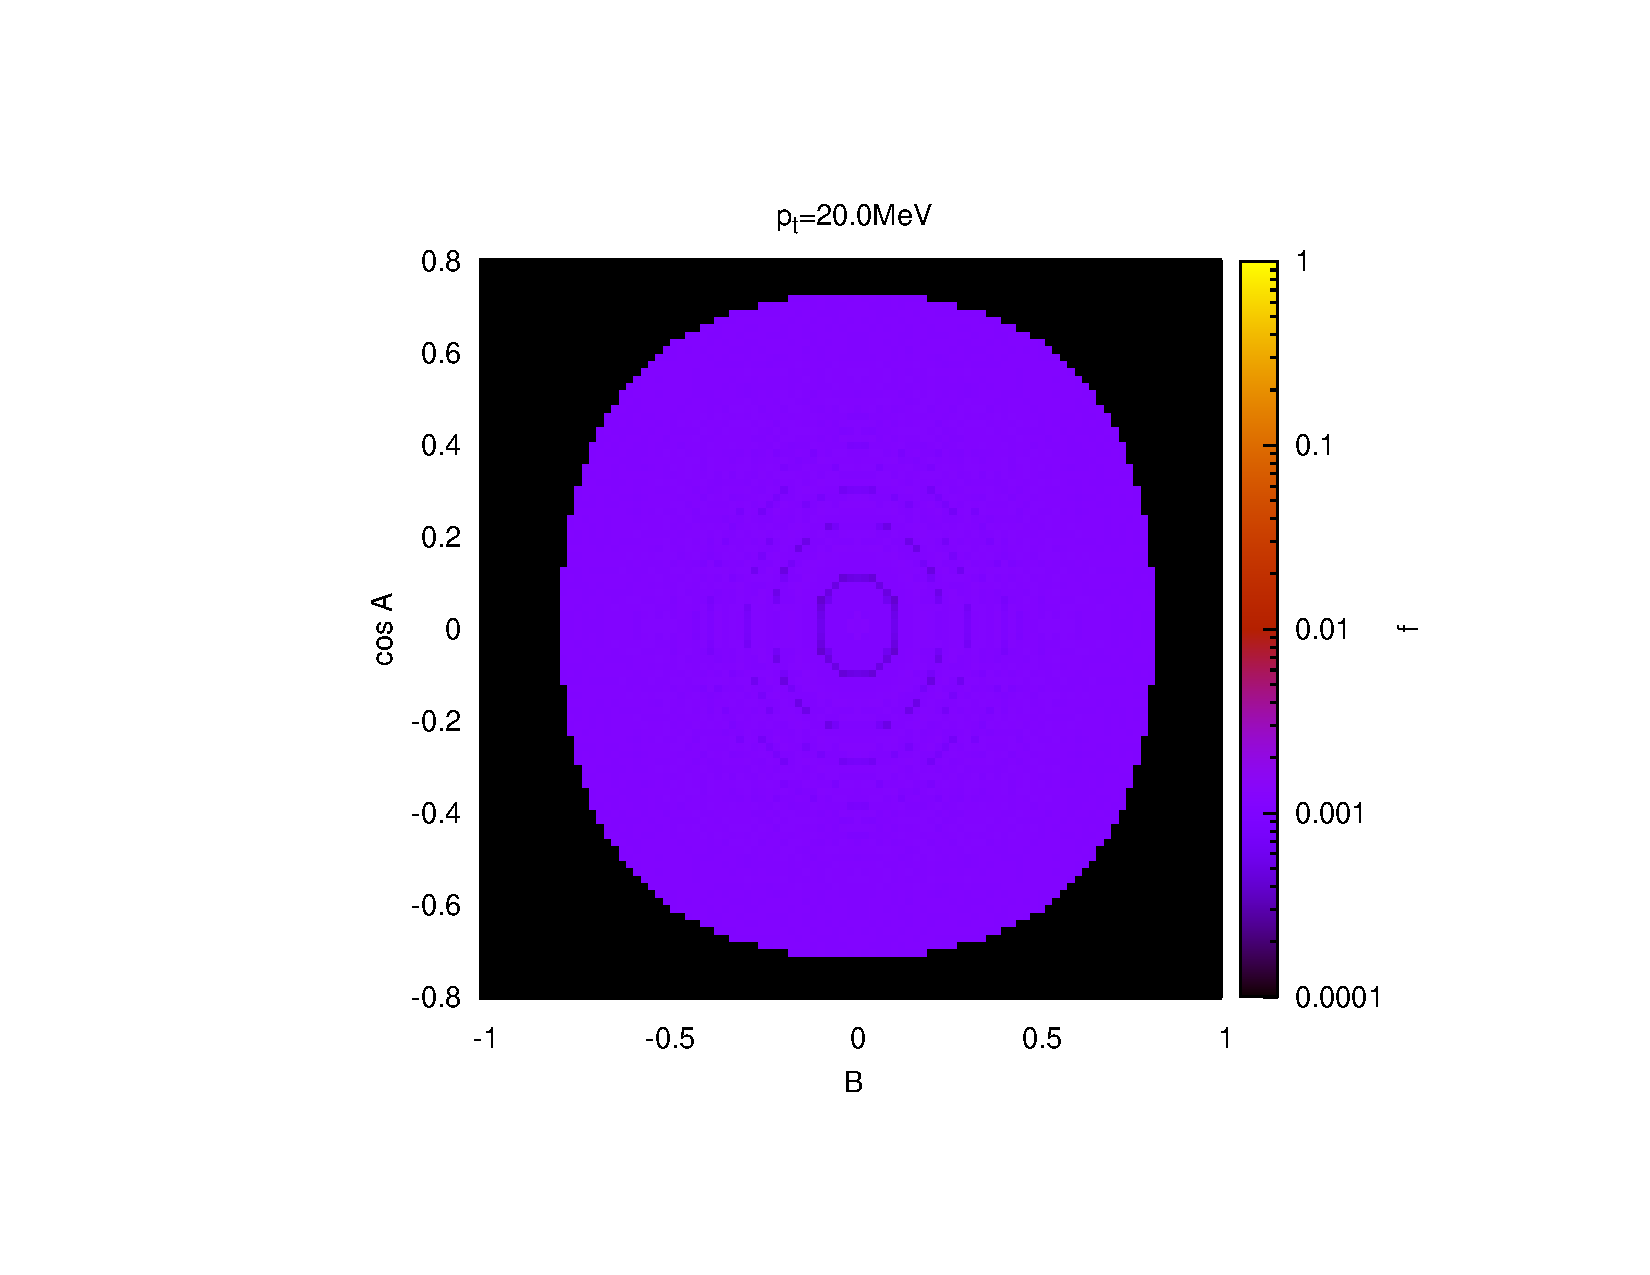
\includegraphics[width=1\linewidth]{Figures/fnue_Alpha_vs_Beta-asano_fukuyama_gr}
  \end{subfigure}
  \begin{subfigure}{.8\textwidth}
    \centering
    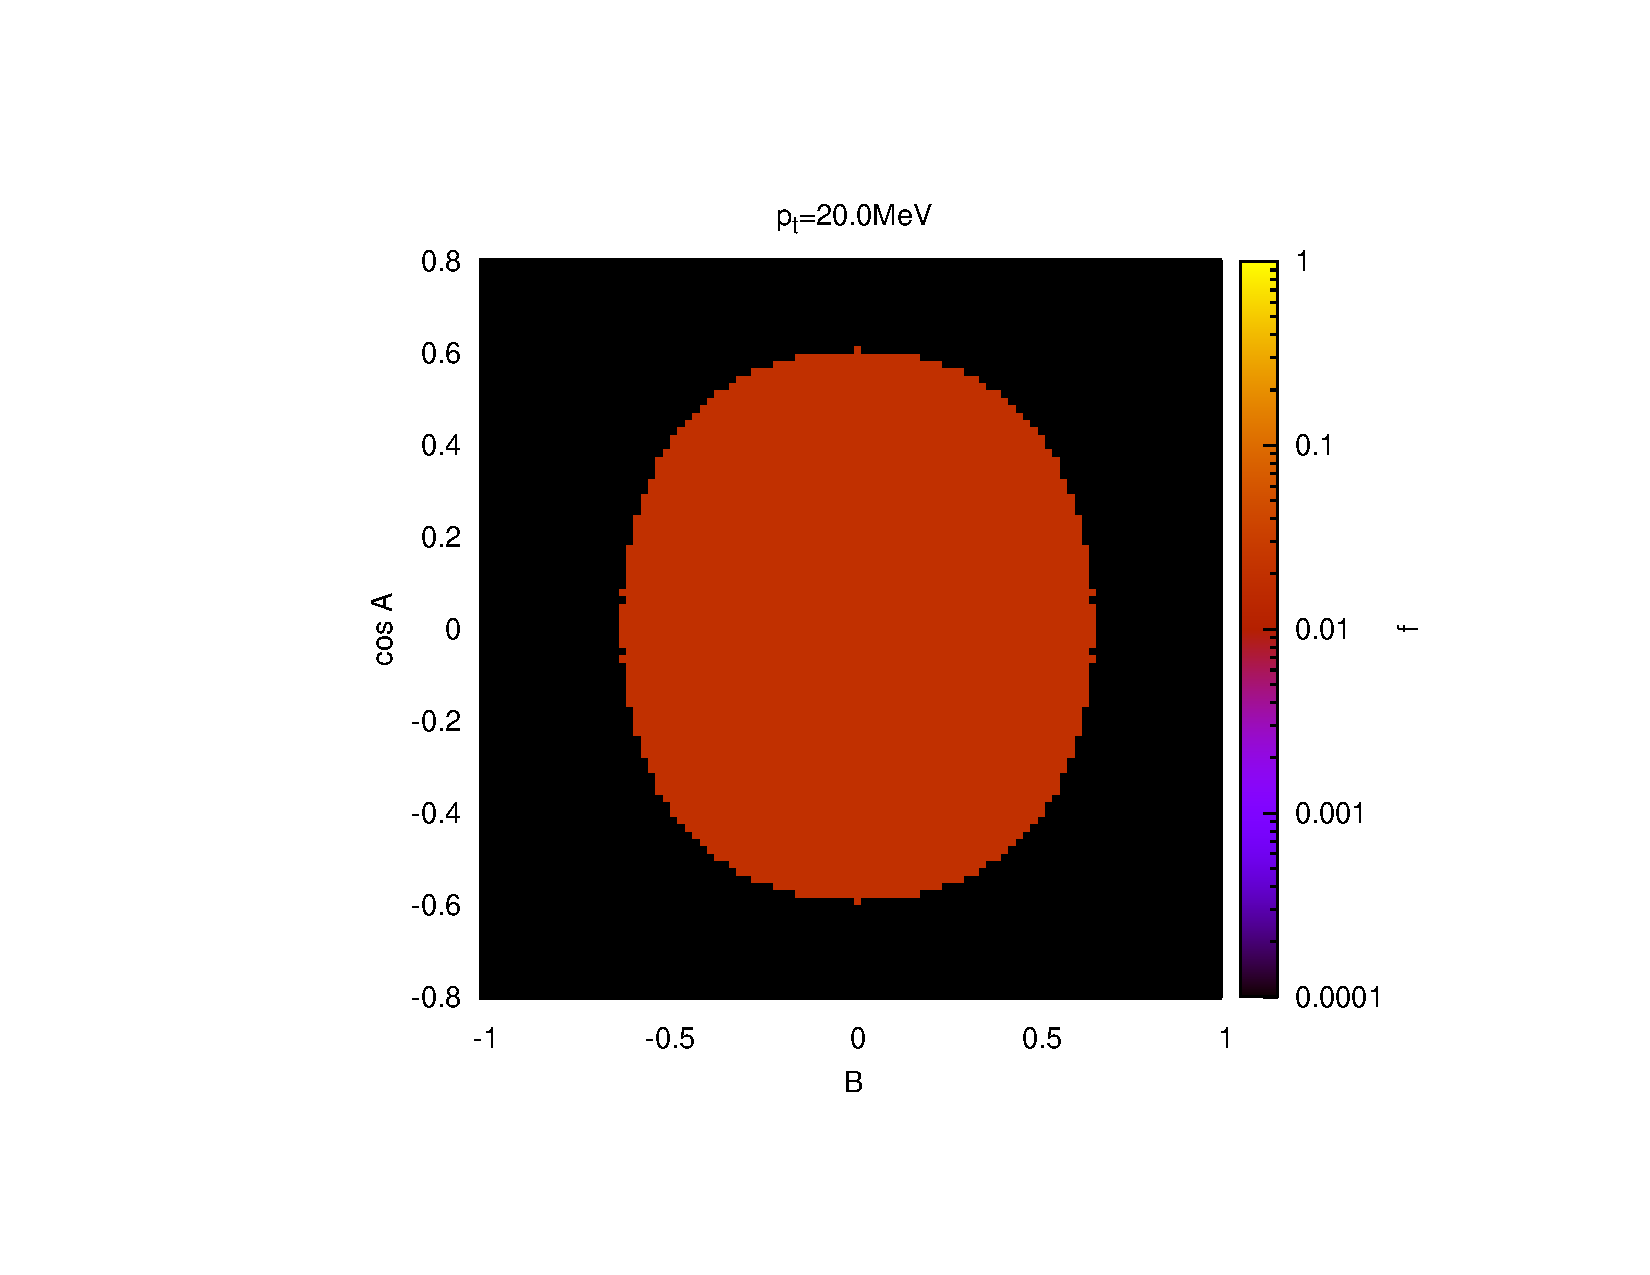
\includegraphics[width=1\linewidth]{Figures/fnue_Alpha_vs_Beta-asano_fukuyama_flat}
  \end{subfigure}
  \caption[$f_\nu$ for a hot compact star: sky map at high energy]{
    $f_\nu$ across a patch of sky in a single energy band, $p_t=20$~MeV.
    The source is a hot compact star: $R_g=2\,M_\odot$, $R_\nu=3\,M_\odot$,
    $T=5$~MeV, and $\eta=0.1$.
    The observer is stationary at Schwarzschild radius $5\,M_\odot$.
    \emph{Top Figure}: Schwarzschild spacetime.
    \emph{Bottom Figure}: Minkowski spacetime.
    These two stars have identical coordinate radii, and identical local fluid
    properties at their neutrinospheres.
  }
  \label{fig:f_hot_ns}
\end{figure}

Fig.~\ref{fig:f_spectrum_hot_ns} presents the energy spectrum emitted by this
surface over the broad band $p_t\in[0.01,100]~MeV$, for both Schwarzschild
and Minkowski cases.
We also show the relative errors in $f_\nu(p_t)$, with respect to the analytic
solution $f_{\nu,\rm ex}(p_t)$. The Minkowski calculation is exact to machine
precision, because location of the neutrinosurface has no effect on $f_\nu$.
But the relative errors in the Schwarzschild case are large, and grow to
20\% at 100~MeV. (It is important to keep in mind that this is not the case
generally, but only when the neutrinosurface is in a steep gravitational
potential.
This will be an important consideration in Sec.~\ref{sec:q_algorithm}:
spectral information at energies near 100~MeV can be important in the
neutrino-antineutrino annihlation calculation because the process depends very
steeply upon the neutrino energies.

\begin{figure}
  \centering
  \begin{subfigure}{.7\textwidth}
    \centering
    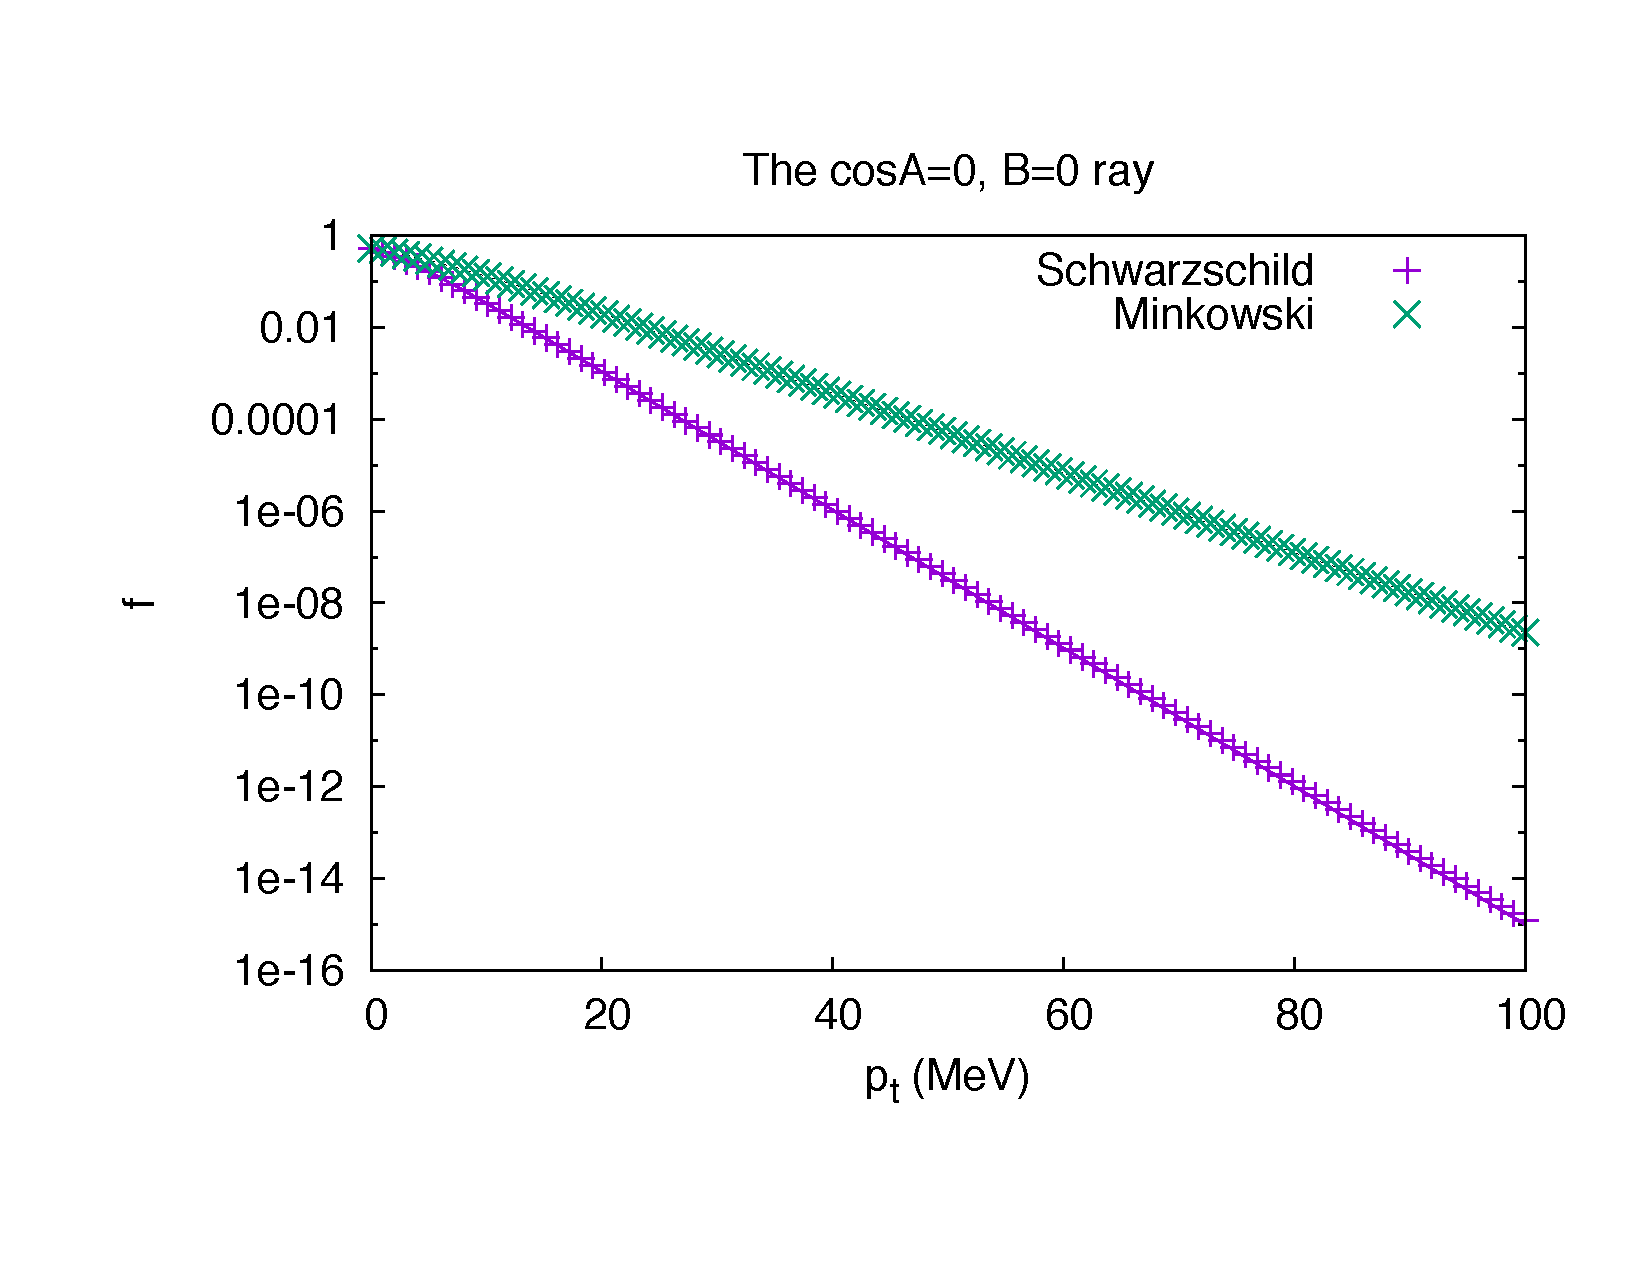
\includegraphics[width=1\linewidth]{Figures/fnue_vs_E-asano_fukuyama}
  \end{subfigure}
  \begin{subfigure}{.7\textwidth}
    \centering
    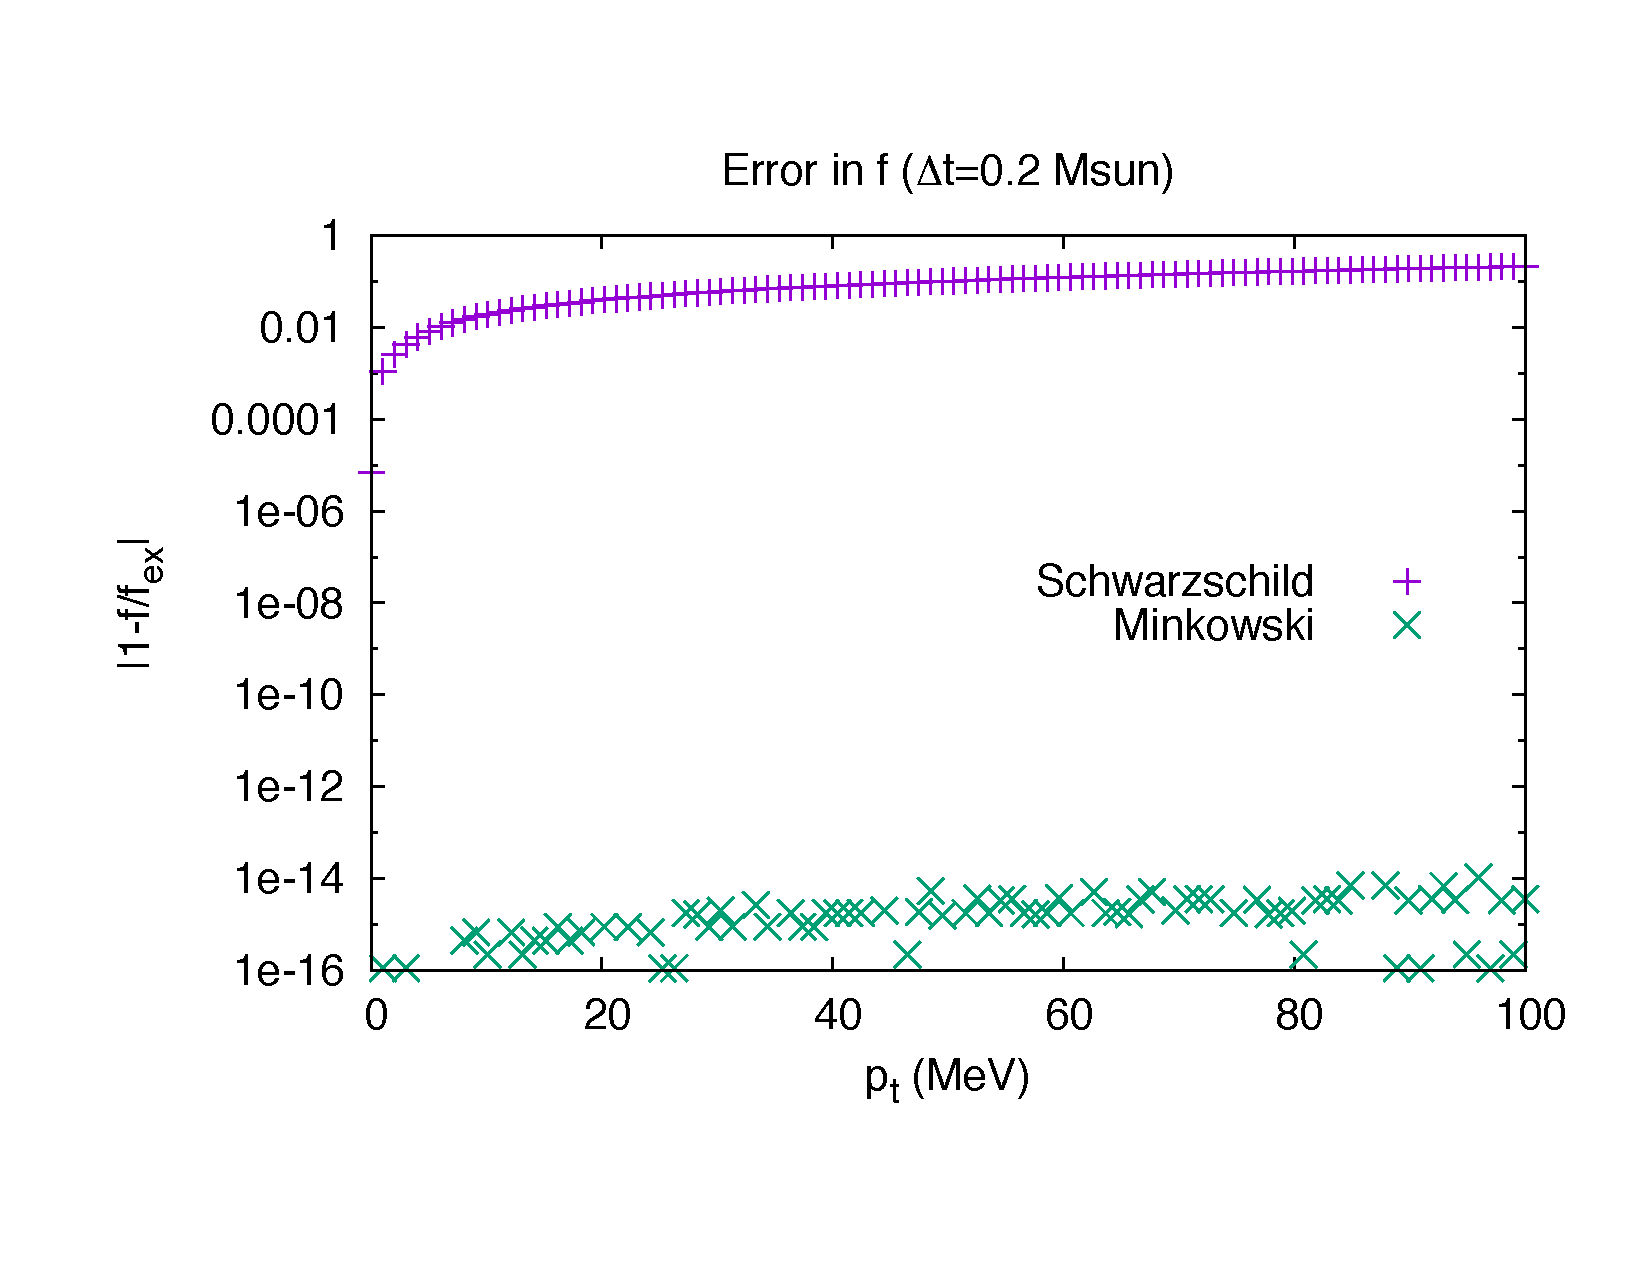
\includegraphics[width=1\linewidth]{Figures/fnueError_vs_E-asano_fukuyama}
  \end{subfigure}
  \caption[$f_\nu$ for a hot compact star: asymptotic energy spectrum]{
    The $p_t$ spectrum of the hot compact star from the same viewing
    position as in Fig.~\ref{fig:f_hot_ns}. These plots show $f_\nu$ sampled by
    the $\cos A=0$, $B=0$ rays.
    \emph{Top Figure}: $f_\nu(p_t)$ in the case of a curved and flat spacetime.
    The exact distribution functions $f_{\nu, \rm ex}(p_t)$ are represented as solid
    lines, which lie directly beneath the data points.
    \emph{Bottom Figure}: The relative error in $f_\nu$ for these two cases.
    For the flat spacetime distribution function, the error bottoms out at
    machine roundoff.
  }
  \label{fig:f_spectrum_hot_ns}
\end{figure}

\section{$f_\nu$ for this Accretion Disk}
\label{sec:f_this_case}

Let us examine the neutrino emission from the post-merger accretion disk model
presented in Chap.~\ref{chap:leakage}. Here we sample $f_\nu$ at two positions,
on the rotation axis and on the equator, about 120~km from the black hole
and at a late time, about 40~ms after merger. At this time the disk has reached
a quasi-equilibrium accretion state, with most of the asymmetry of the merger
having been smeared out by differential rotation, making the model ideal for our
time-independent ray tracing approximation. The disk's luminosity in neutrinos
has decayed to approximately $10^{53}$~erg~s$^{-1}$
(Fig.~\ref{fig:globalevolution}). In this sense, our later calculation of
neutrino-antineutrino annihilation power will provide a lower bound for energy
available to drive a jet.

In fact, 40~ms after a realistic merger with these bulk parameters, we expect
magnetic effects to play a significant role in the accretion dynamics,
\todo{cite someone}
increasing the accretion rate via the magneto-rotational instability, and heating
the disk through a turbulent transport of energy from large scales (bulk kinetic
energy) to small scales (random thermal energy). In this model we neglect this
important physics, and again, in this sense, our later neutrino-antineutrino
annihilation power calculation will provide a lower bound on jet energetics.

\subsubsection{From the Rotation Axis}
\label{sssc:f_this_case_A}

In Figs.~\ref{fig:f_disk_axis_13MeV}~and~\ref{fig:f_disk_axis_34MeV} I display
$f_\nu(\Omega_i)$ over the whole sky, as viewed from the rotation axis, at the
characteristic energies of 13~MeV and 34~MeV. These figures are analagous to
Fig.~\ref{fig:f_hot_ns}. I've sampled $f_\nu$ at these energies because the first is
near the average neutrino energy (see for example
Fig.~\ref{fig:neutrinos_by_species}), and the latter gives us a feel for the
angular distribution of high-energy emission. At lower energies our opaque
disk assumption begins to break down: the disk is transparent to neutrinos at
energies $\lesssim5$~MeV.
\todo{confirm, cite later $\nu\bar{\nu}$ discussion of energy bounds}

All three species of neutrinos represented in the leakage scheme are represented
in these figures: $\nu_e$, $\nu_a \equiv \bar{\nu}_e$, and
$\nu_x \equiv \{\nu_\mu,\bar{\nu}_\mu,\nu_\tau,\bar{\nu}_\tau\}$.

\begin{figure}
  \centering
  \begin{subfigure}{.3\textwidth}
    \centering
    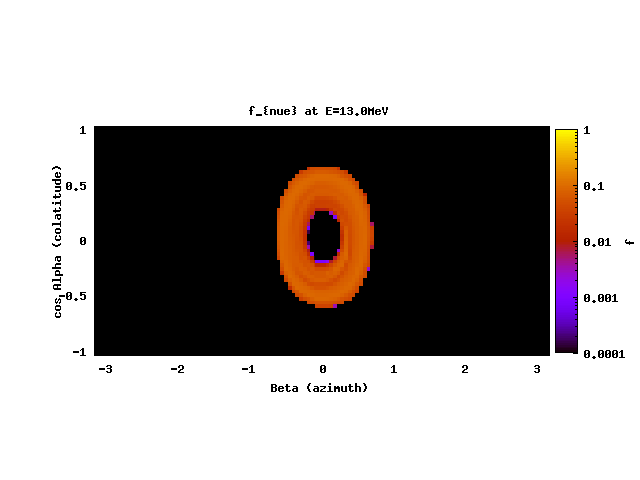
\includegraphics[width=1\linewidth]{Figures/f_nue-A-13MeV}
  \end{subfigure}
  \begin{subfigure}{.3\textwidth}
    \centering
    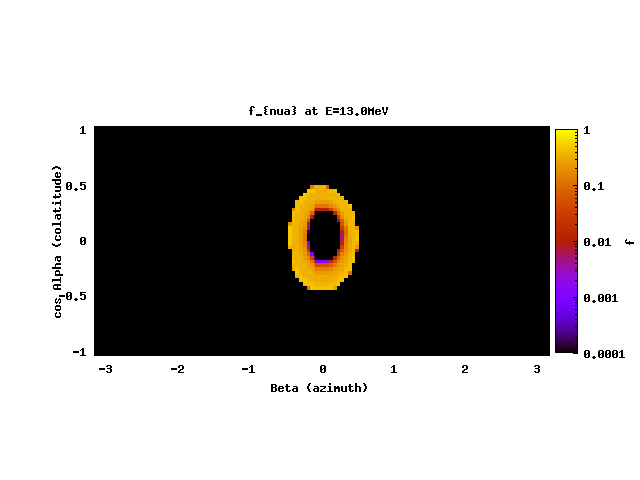
\includegraphics[width=1\linewidth]{Figures/f_nua-A-13MeV}
  \end{subfigure}
  \begin{subfigure}{.3\textwidth}
    \centering
    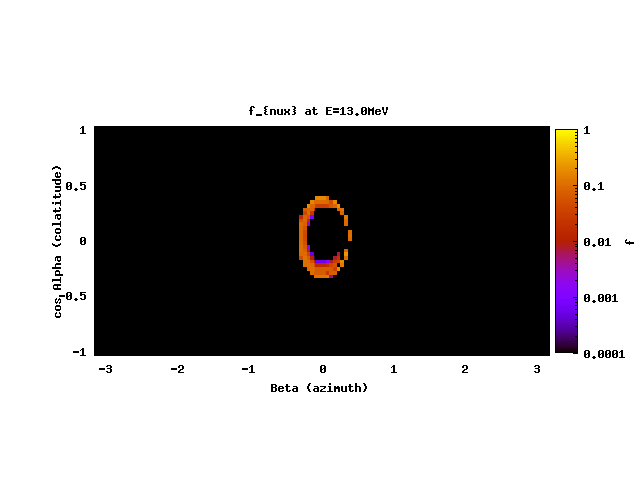
\includegraphics[width=1\linewidth]{Figures/f_nux-A-13MeV}
  \end{subfigure}
  \caption[$f_\nu$ for the disk, from the rotation axis: sky map at average energy]{
    Neutrino distribution functions from the accretion disk over the sky in a
    single energy band, $p_t=13$~MeV. The observer is stationary on the rotation
    axis at coordinate radius 120~km from the black hole. The panels from
    left to right depict $f_{\nu_e}$, $f_{\nu_a}$, $f_{\nu_x}$.
  }
  \label{fig:f_disk_axis_13MeV}
\end{figure}

\begin{figure}
  \centering
  \begin{subfigure}{.3\textwidth}
    \centering
    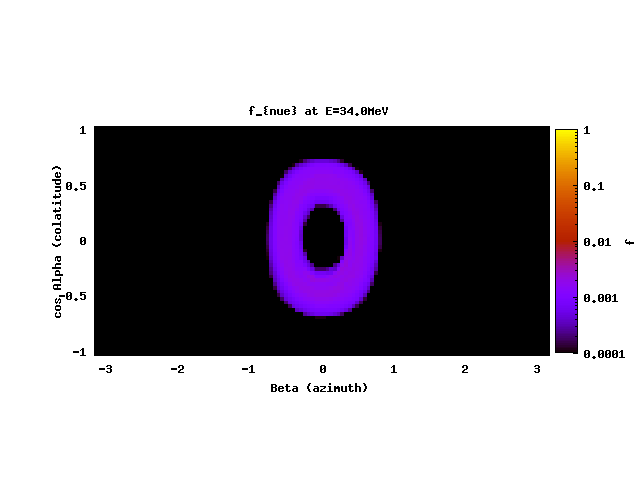
\includegraphics[width=1\linewidth]{Figures/f_nue-A-34MeV}
  \end{subfigure}
  \begin{subfigure}{.3\textwidth}
    \centering
    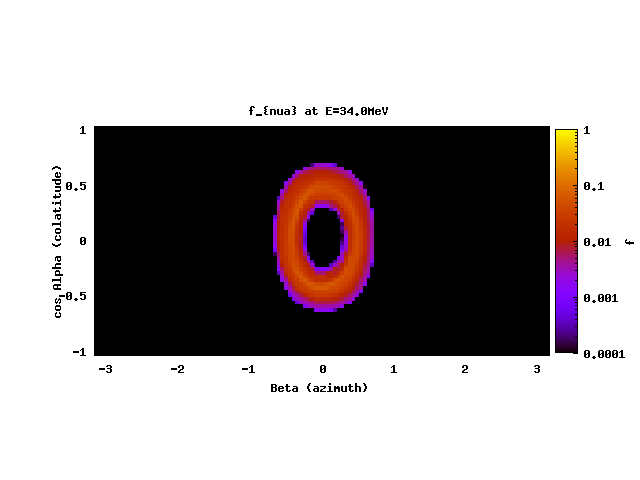
\includegraphics[width=1\linewidth]{Figures/f_nua-A-34MeV}
  \end{subfigure}
  \begin{subfigure}{.3\textwidth}
    \centering
    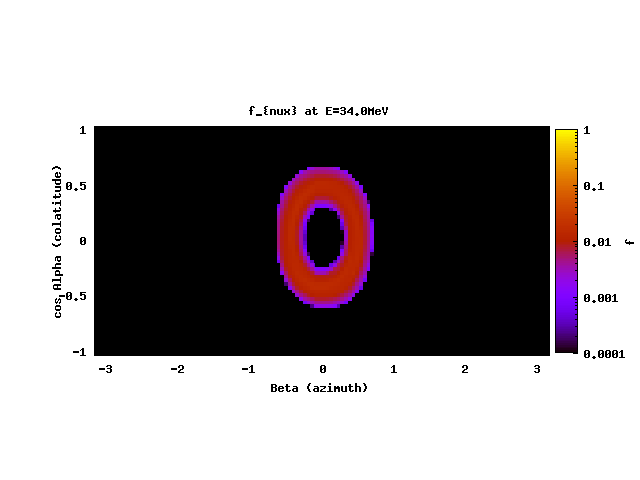
\includegraphics[width=1\linewidth]{Figures/f_nux-A-34MeV}
  \end{subfigure}
  \caption[$f_\nu$ for the disk, from the rotation axis: sky map at high energy]{
    Same as Fig.~\ref{fig:f_disk_axis_13MeV}, but in the energy band $p_t=34$~MeV.
    Left to right, the panels depict $f_{\nu_e}$, $f_{\nu_a}$, and $f_{\nu_x}$.
  }
  \label{fig:f_disk_axis_34MeV}
\end{figure}

Several observations:
\begin{enumerate}
  \item The neutrino surface is larger at higher energy.
    This is because of the opacities' energy dependence,
    $\chi\propto\varepsilon^2$. The higher-energy neutrinosurfaces are further
    away from the black hole, where redshift effects are smaller, than the
    lower-energy neutrinosurfaces. Thus, we may infer that a realistic neutrino
    spectrum is suppressed at low energy compared to that obtained from a
    simple Newtonian calculation.
  \item The brightest ring of emission is not at the extreme inner edge, even
    though the disk temperature is consistently high all the way to the inner
    edge (see for example Fig.~\ref{fig:profiles}). This is a straightforward
    effect of the stronger redshift operating near the black hole.
  \item $f_{\nu_a}$ is brighter than $f_{\nu_e}$
    and emitted from a smaller region.
    \label{item:zeta}
    This is because the disk is less opaque
    to $\bar{\nu}_e$ (see Fig.~\ref{fig:zeta_meridional}). The dominant
    charged-current processes make this clear: in a neutron-rich fluid like that
    of this disk (again see Fig.~\ref{fig:profiles}), $\nu_e$ absorption via
    $\nu_e\,n \rightarrow p\,e^{-}$
    is favored over $\bar{\nu}_e$ absorption via
    $\bar{\nu}_e\,p \rightarrow n\,e^{+}$.
    So the $\bar{\nu}_e$s decouple from the fluid from deeper within the disk,
    at a hotter temperature, and are therefore more luminous.
  \item The $\nu_a$- and $\nu_x$-surfaces are sharp-edged at low energy,
    with little sign of the limb-darkening seen in the $\nu_e$ surfaces.
    \label{item:eta}
    This is perhaps an unrealistic effect of our choice of leakage neutrino
    chemical potentials, described in Sec.~\ref{sec:leakage}.

    In the leakage scheme, $\eta_{\nu_i}$ is calculated using local fluid
    properties and a rough estimate of whether the neutrinos at that location are
    trapped or free: $\langle \tau_{\nu_i} \rangle$, the energy-averaged optical
    depth.
    This skews the ray tracing calculation of $f_\nu$ at energies very different
    than $\langle \varepsilon_{\nu_i} \rangle$.
    %At energies below
    %$\langle \varepsilon_{\nu_i} \rangle$, the neutrinosurface found by ray
    %tracing will be deep in the disk, where the leakage scheme estimated
    %the neutrinos to be trapped. Whether this amplifies or suppresses the
    %emission depends on the local fluid properties at the neutrinosurface.
    Deep in the disk, where $\langle \tau_{\nu_i} \rangle \gtrsim 1$,
    $\eta_{\nu_e}$ and $\eta_{\nu_a}$ are calculated by assuming equilibrium
    of the charged current reactions described in observation~\ref{item:zeta},
    so that $\eta_{\nu_e}=-\eta_{\nu_a}$.
    Also, due to the $n$-richness of the disk, $\eta_{\nu_e}<\eta_{\nu_a}$.
    These two conditions for the neutrino chemical potentials constrain
    $\eta_{\nu_a}>0$ deep in the disk, as can be seen in
    Fig.~\ref{fig:eta_meridional}.
    This amplifies $f_{\nu_a}$ at low energies.

    (Note, because of lower interaction rates for heavy lepton neutrinos,
    $\eta_{\nu_x}$ is set identically to zero in our leakage approximation.)
    \todo{why does this make $f_\nu$ sharp?}
  \item $f_{\nu_a}$ and $f_{\nu_x}$ appear similar at these two energies.
    This may be a special coincidence of this late time, when $\nu_a$ and
    $\nu_x$ opacities are similar (see Fig.~\ref{fig:zeta_meridional}).

    In fact, if these two distribution functions
    are similar across the entire energy spectrum (I have not yet examined this,
    but it's likely since the opacities are smooth fields in the disk),
    the luminosities estimated by ray tracing and leakage would be
    inconsistent (see Fig.~\ref{fig:neutrinos_by_species}).

    %We expect $\nu_x$ to decouple from the fluid deeper in the disk than
    %the $e$-type neutrinos, because the disk is less opaque to the former.
    %The only scattering processes for $\nu_x$ at these energies involve
    %neutral-current weak interactions, to which $e$-type neutrinos are also
    %subject. But the The $e$-type neutrinos additionally have the power to
    %interact with nuclear matter via charged-current processes.
    %Only at unphysically high energies ($m_{\mu}\sim100$~MeV,
    %$m_{\tau}\sim2$~GeV) do the charged current processes become available to
    %the heavy-lepton neutrinos.
    %\todo{is this true?}
    %So the similarity of $f_{\nu_a}$ and $f_{\nu_x}$ raises a suspicion about
    %this calculation.

    However, our use of leakage chemical potentials to construct the neutrino
    distribution functions (as discussed in observation~\ref{item:eta}) may contribute
    to the similarity of these two $f_\nu$s. Even though the $\nu_x$-surface is
    a little deeper in the disk and at a slightly higher temperature than the
    $\nu_a$-surface (effectively boosting $\nu_x$ emission),
    its chemical potential is lower (effectively suppressing $\nu_x$ emission).
    In this case, at this late time, the two effects approximately cancel.

    As this observation highlights, the leakage and ray tracing estimates of
    neutrino luminosity are not self-consistent by construction: they are
    different approximations. The former accounts for local energy losses
    throughout the fluid volume, the latter accounts for energy losses from a
    surface.
\end{enumerate}

\begin{figure}
  \centering
  \begin{subfigure}{.31\textwidth}
    \centering
    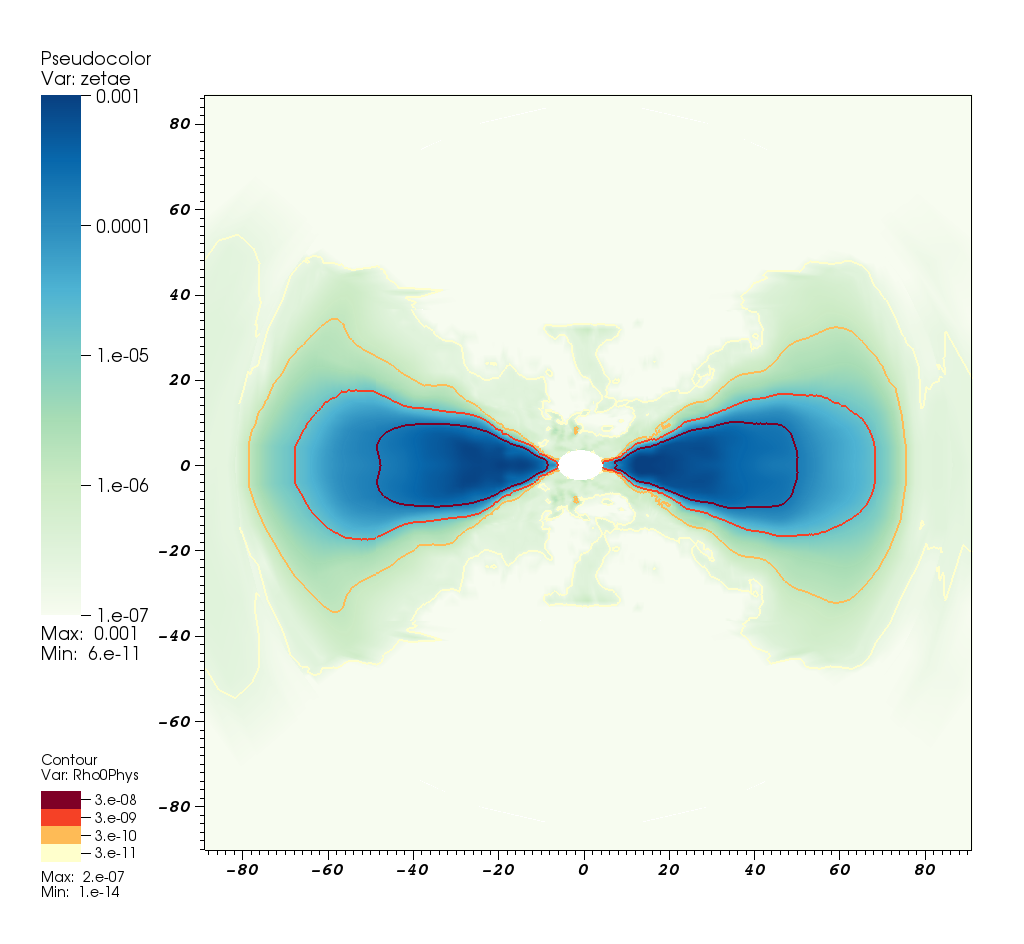
\includegraphics[width=1\linewidth]{Figures/zetae_meridional}
  \end{subfigure}
  \begin{subfigure}{.31\textwidth}
    \centering
    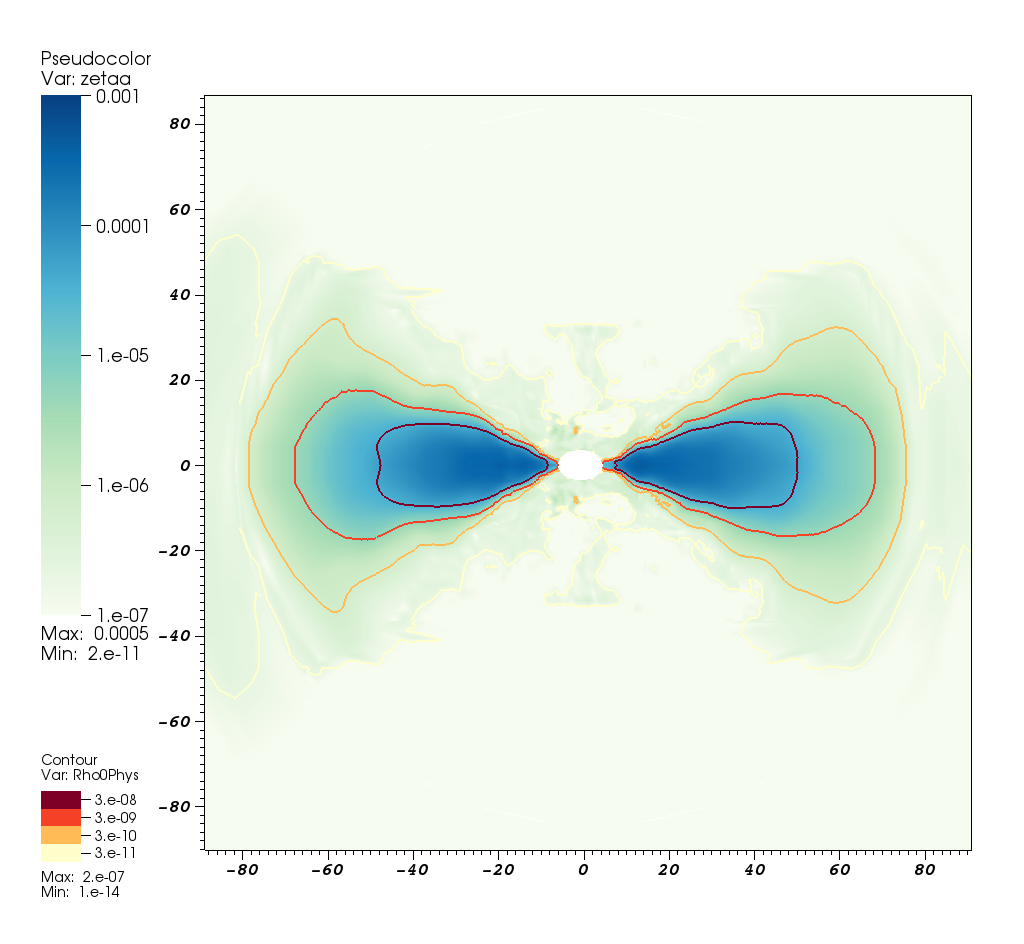
\includegraphics[width=1\linewidth]{Figures/zetaa_meridional}
  \end{subfigure}
  \begin{subfigure}{.31\textwidth}
    \centering
    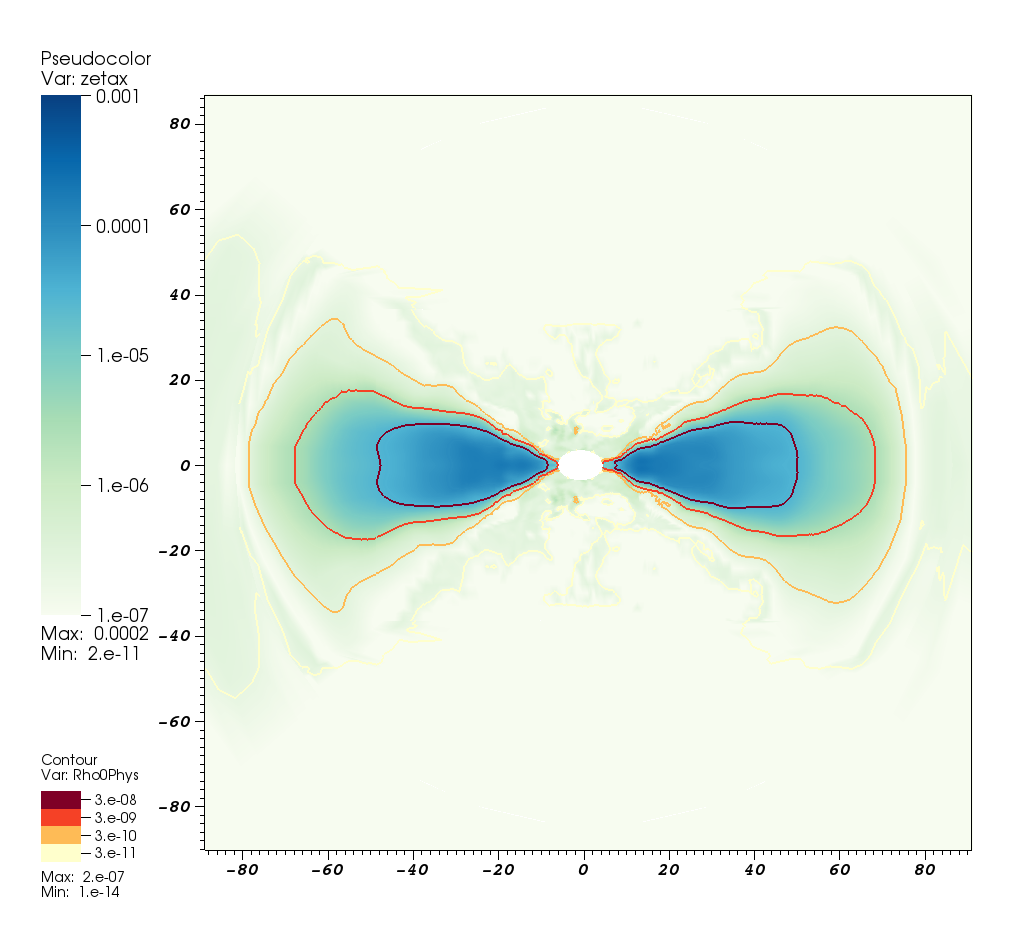
\includegraphics[width=1\linewidth]{Figures/zetax_meridional}
  \end{subfigure}
  \caption[Disk opacities]{
    Meridional slices of disk opacities for each neutrino species,
    $\zeta_{\nu_i}$, in geometrized units of $M_\odot^{-2}$~MeV$^{-1}$.
    The axes are labeled in units of $M_\odot\sim1.5$~km.
    Decadal density contours, in units of $M_\odot^{-2}\sim10^{18}$~g~cm$^{-3}$,
    are provided to give a sense of the matter distribution.
  }
  \label{fig:zeta_meridional}
\end{figure}

\begin{figure}
  \centering
  \begin{subfigure}{.31\textwidth}
    \centering
    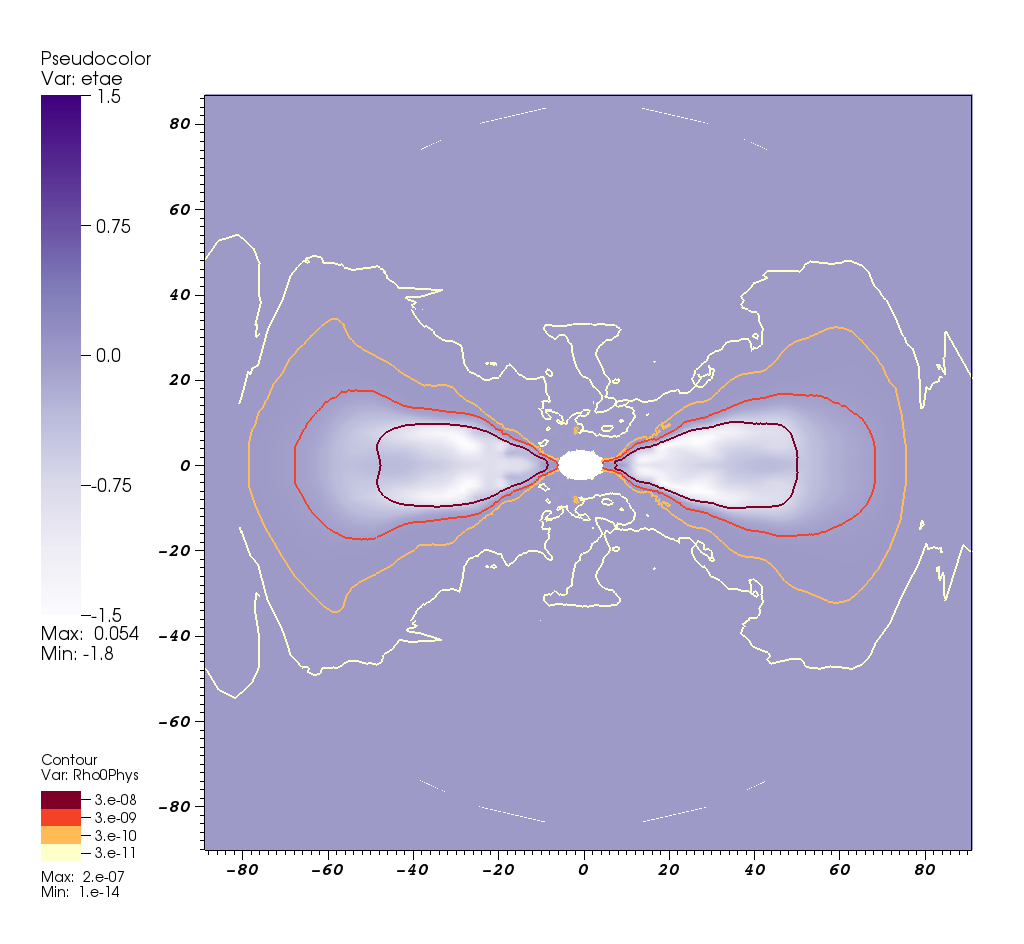
\includegraphics[width=1\linewidth]{Figures/etae_meridional}
  \end{subfigure}
  \begin{subfigure}{.31\textwidth}
    \centering
    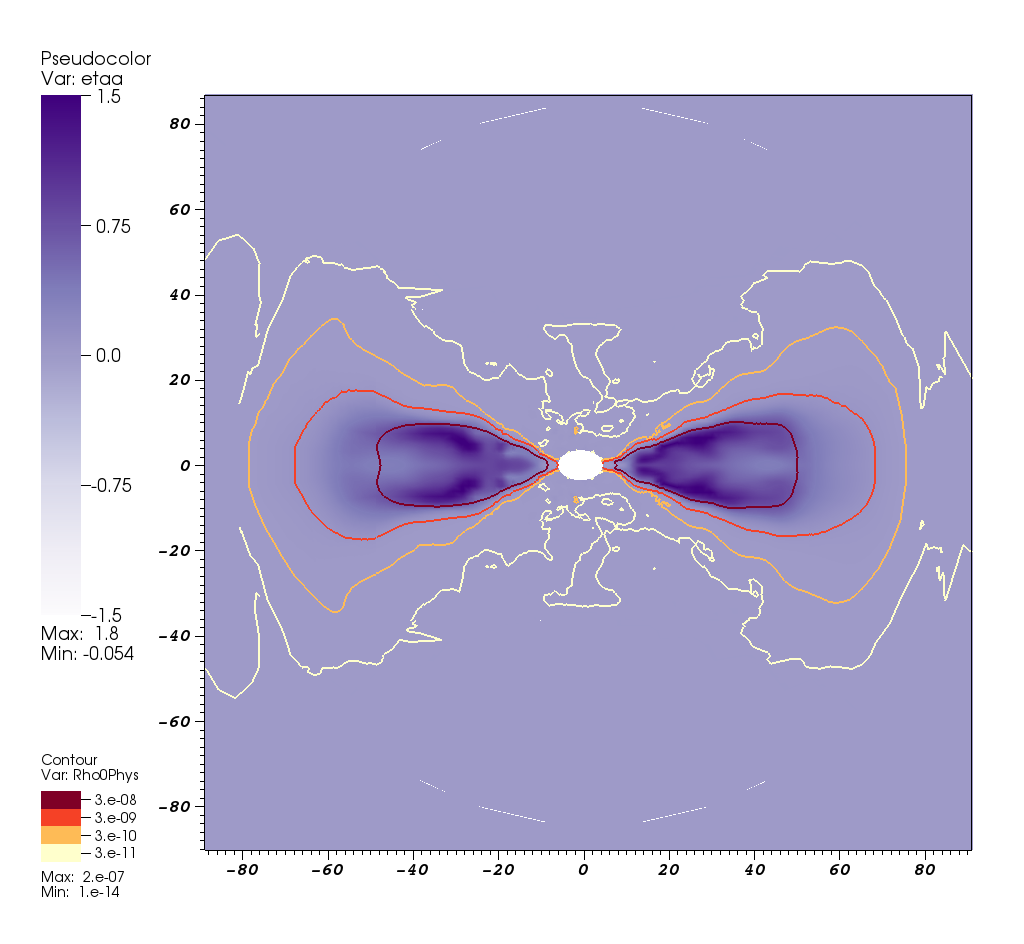
\includegraphics[width=1\linewidth]{Figures/etaa_meridional}
  \end{subfigure}
  \caption[Disk neutrino chemical potentials]{
    Meridional slices of neutrino chemical potentials for $\nu_e$ and
    $\nu_a$. The chemical potential for $\nu_x$ is zero by construction
    in the leakage scheme: the heavy-lepton neutrinos are assumed to
    stream freely.
    The axes are labeled in units of $M_\odot\sim1.5$~km.
    Decadal density contours, in units of $M_\odot^{-2}\sim10^{18}$~g~cm$^{-3}$,
    are provided to give a sense of the matter distribution.
  }
  \label{fig:eta_meridional}
\end{figure}

\subsubsection{From the Equator}
\label{sssc:f_this_case_E}

In Figs.~\ref{fig:f_disk_eq_13MeV}~and~\ref{fig:f_disk_eq_34MeV} I display
$f_\nu(\Omega_i)$ over the whole sky, as viewed from the equator, at the
same characteristic energies as in
Figs.~\ref{fig:f_disk_axis_13MeV}~and~\ref{fig:f_disk_axis_34MeV}.

\begin{figure}
  \centering
  \begin{subfigure}{.3\textwidth}
    \centering
    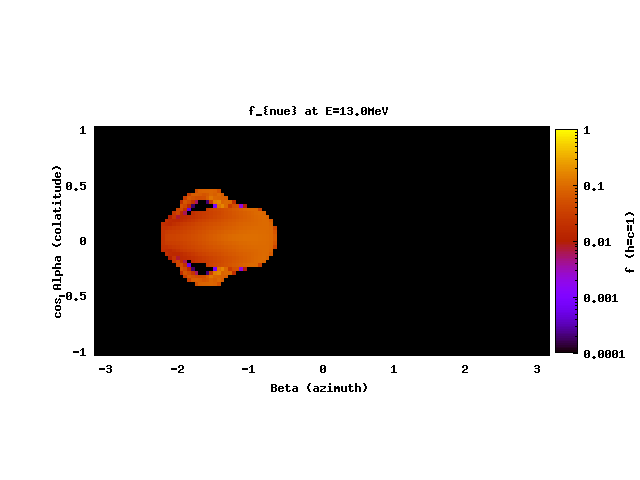
\includegraphics[width=1\linewidth]{Figures/f_nue-E-13MeV}
  \end{subfigure}
  \begin{subfigure}{.3\textwidth}
    \centering
    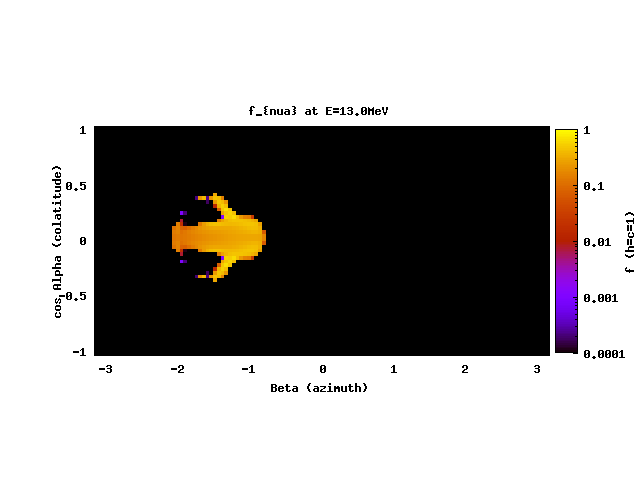
\includegraphics[width=1\linewidth]{Figures/f_nua-E-13MeV}
  \end{subfigure}
  \begin{subfigure}{.3\textwidth}
    \centering
    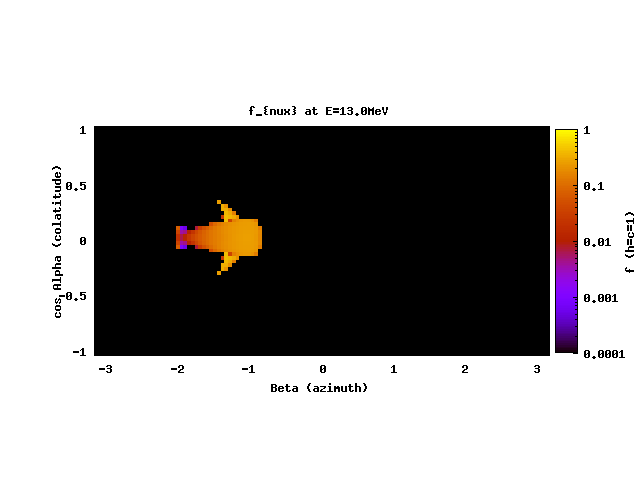
\includegraphics[width=1\linewidth]{Figures/f_nux-E-13MeV}
  \end{subfigure}
  \caption[$f_\nu$ for the disk, from the equatorial plane: sky map at average energy]{
    Neutrino distribution functions from the accretion disk over the sky in a
    single energy band, $p_t=13$~MeV. The observer is stationary in the
    equatorial plane at coordinate radius 120~km from the black hole.
    The panels from left to right depict $f_{\nu_e}$, $f_{\nu_a}$,
    and $f_{\nu_x}$.
  }
  \label{fig:f_disk_eq_13MeV}
\end{figure}

\begin{figure}
  \centering
  \begin{subfigure}{.3\textwidth}
    \centering
    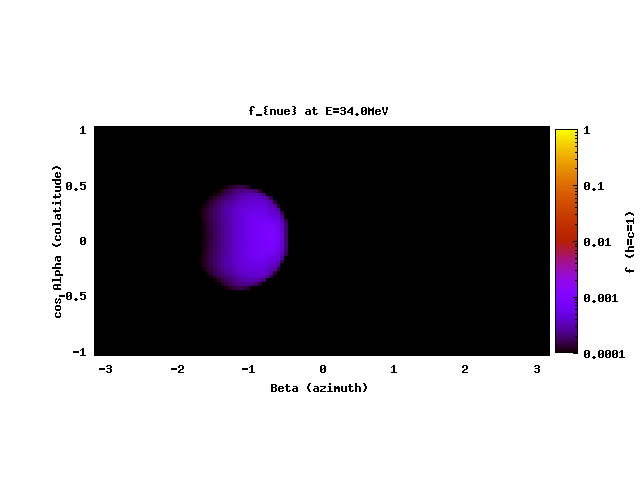
\includegraphics[width=1\linewidth]{Figures/f_nue-E-34MeV}
  \end{subfigure}
  \begin{subfigure}{.3\textwidth}
    \centering
    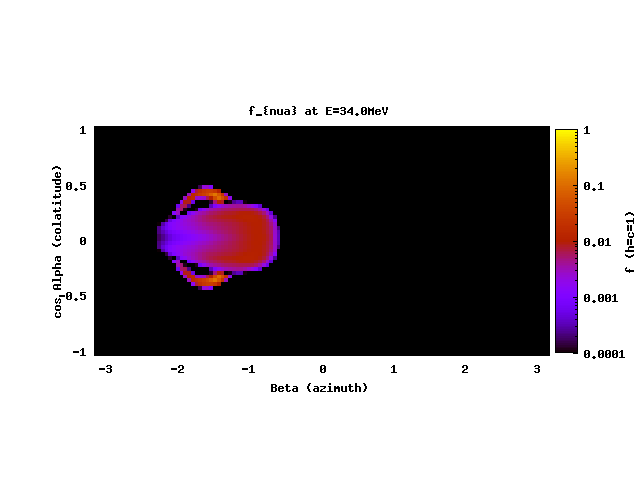
\includegraphics[width=1\linewidth]{Figures/f_nua-E-34MeV}
  \end{subfigure}
  \begin{subfigure}{.3\textwidth}
    \centering
    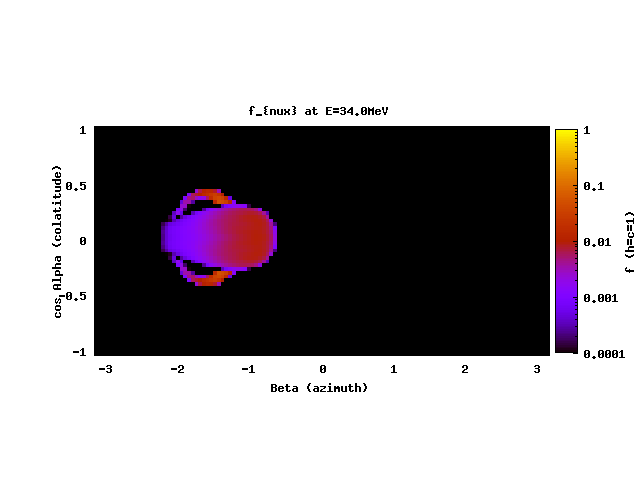
\includegraphics[width=1\linewidth]{Figures/f_nux-E-34MeV}
  \end{subfigure}
  \caption[$f_\nu$ for the disk, from the equatorial plane: sky map at high energy]{
    Same as Fig.~\ref{fig:f_disk_eq_13MeV}, but in the energy band $p_t=34$~MeV.
    Left to right, the panels depict $f_{\nu_e}$, $f_{\nu_a}$, and $f_{\nu_x}$.
  }
  \label{fig:f_disk_eq_34MeV}
\end{figure}

Several observations:
\begin{enumerate}
  \item The back side of the neutrinosurface, behind the black hole, is visible
    as a ring on the top and bottom of the image.
    This is due to the bending of rays by the spacetime curvature of the black
    hole. This has the effect of enlarging the emission surface compared to
    that obtained by a simple Newtonian calculation, an effect seen even in
    the simple case of the hot compact star (Fig.~\ref{fig:f_hot_ns}).
    See Fig.~\ref{fig:schematic_ray_bending} for an explanatory cartoon.
  \item The left side of the neutrinosurface---which is actually the right
    side of the disk in physical space (the image is reflected vertically and
    horizontally, as by a pinhole camera)---is less intense. In the cases of
    $f_{\nu_a}$ and $f_{\nu_x}$, it actually vanishes at low energy.
    This is due to the relativistic fluid velocities: the left side of the disk
    image is moving away from, and the right side toward the viewer.
    See Fig.~\ref{fig:schematic_ray_doppler} for an explanatory cartoon.
    Neutrinos emitted from the left side are doppler shifted to lower energies
    than those from the right side. At these energies,
    $p_t\gtrsim\langle\varepsilon_\nu\rangle$,
    this has the effect of decreasing the intensity, i.e.\ decreasing
    $f_\nu(p_t)$.
    The effect is reversed at energies for which
    $\partial_{p_t}f_\nu(p_t)>0$.
  \item The image of the disk is offset to the left. This is an effect of the
    rotation of the central black hole, which communicates a sympathetic spin
    to the spacetime. This is a well-known and experimentally-verified effect
    \todo{ref theory and GravB}
    called frame dragging, or gravitomagnetism.
    According to a viewer at rest very far away from the disk, neutrinos
    streaming away from its surface follow trajectories curving away from
    the spin of the black hole, forming a whirlpool shape.
    \todo{add cartoon or computed ray trajectories}
\end{enumerate}

\begin{figure}
  \centering
  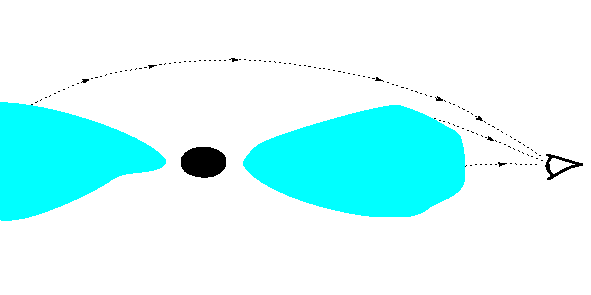
\includegraphics[width=10cm]{Figures/seeing_back_of_disk}
  \caption[Cartoon of neutrino rays bending over the disk]{
    Cartoon showing how a viewer (on the right) can see parts of the
    neutrinosurface that would be obscured in Euclidean geometry.
    This is a meridional slice of the disk. The fluid is shown in blue, the
    black hole is black, and several neutrino trajectories are shown as dashed
    lines.
  }
  \label{fig:schematic_ray_bending}
\end{figure}

\begin{figure}
  \centering
  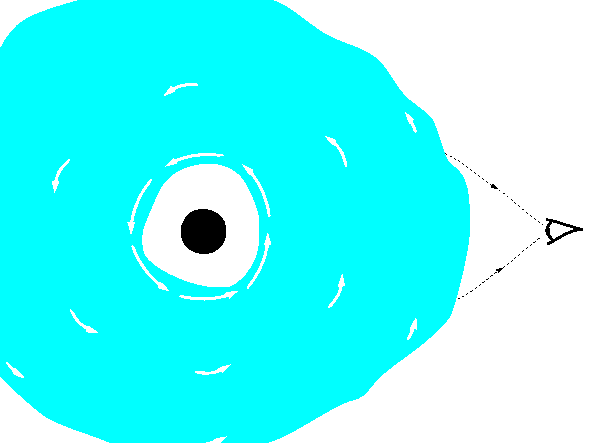
\includegraphics[width=10cm]{Figures/seeing_disk_doppler_shift}
  \caption[Cartoon of the doppler shift due to disk rotation]{
    Cartoon showing how a viewer (on the right) experiences a differential
    doppler shift. This is an equatorial slice of the disk.
    The fluid is shown in blue and its velocity field by white arrows, longer
    representing faster. The black hole is black, and two neutrino trajectories
    are shown as dashed lines. The left side of the disk (downward in the
    cartoon) is moving roughly toward the viewer, boosting its neutrino emission;
    the opposite is true of the right side of the disk.
    Furthermore, the differential rotation of the disk makes this effect more
    pronounced for neutrinosurfaces deeper within the disk.
  }
  \label{fig:schematic_ray_doppler}
\end{figure}

\section{Calculating $q_{\nu \bar{\nu}}$}
\label{sec:q_algorithm}
The standard model for gamma ray bursts consists of an ultrarelativistic jet
driven by rapid accretion onto a stellar-mass black hole. One of the missing
links in this model is the physical mechanism connecting the accretion to the
jet. How does the gravitational energy released by the transport of matter
toward and eventually into the black hole end up powering a highly-collimated
low-density plasma moving away from the black hole with a Lorentz factor of
10s or 100s? The link likely takes the form of one or both of the following
processes:
\begin{itemize}
  \item \emph{Magnetic fields}: If there are strong magnetic fields present, the
    Blandford-Znajek process \citep{blan1977-blandford_znajek} can extract
    rotational energy from the black hole and accelerate plasma out along its
    rotation axis. Additionally, magnetic fields in the accretion disk may
    centrifugally accelerate plasma, tapping the rotational energy of the
    disk itself \citep{blan1982-blandford_payne}.
  \item \emph{Neutrino heating}: Highly energetic neutrino-antineutrino pairs
    can annihilate into into electron-positron pairs
    ($\nu \, \bar{\nu} \rightarrow e^{-} \, e^{+}$)
    with excess energy from the interaction going into the kinetic energy of the
    lepton pair.
    This process is particularly efficient at high neutrino energies and large
    collision angles, conditions found in the funnel of the accretion disk.
    This $e^{-}\,e^{+}$ gas rapidly thermalizes via electromagnetic interactions,
    and the superheated plasma expands away from the disk explosively. The inner
    walls of the funnel may act to confine the plasma, collimating it into a jet.
\end{itemize}

Simulations indicate that the first process is extremely sensitive to the
\todo{ask fatemeh for ref}
initial magnetic field configuration, with no jet structure forming if there is
no initially large-scale poloidal field in the accretion disk.
I won't explore the magnetic processes further here.

The second process is sensitive to the geometry and spectrum of the emission
\todo{cite geneology of $\nu\bar{\nu}$ studies}
and in the context of neutron star--black hole mergers, has only been studied
in highly-idealized models of analytical accretion disks or Newtonian gravity.
\todo{maybe add technical specs of GRBs and nuclear accretion sites}

Let us explore the viability of the neutrino-antineutrino annihilation process
in the case of the accretion disk presented in Chap.~\ref{chap:leakage}.

\subsubsection{Brief History of Neutrino-Antineutrino Annihilation Studies}
\label{sssc:nunubar_review}
In the late 1980s, \cite{good1987-nunubar} and \cite{bere1987-nunubar}
independently proposed neutrino-antineutrino annihilation as a process that could
transfer a fraction of the neutrino energy released by stellar collapse, as in
Type II supernovae, into an electron-positron pair plasma. Their calculations
were performed assuming Newtonian gravity, but they found efficiencies of a
fraction of a percent of the total neutrino luminosity.
\todo{add paczynski 1990}
\todo{add Meszaros \& Rees 1992}

\cite{salm1999-nunubar} examined the same process in a general relativistic
formulation and discovered an enhancement of efficiency to a few percent.
They assumed a Schwarzschild geometry, a spherical emitter, and a Fermi-Dirac
\todo{check}
neutrino spectrum.

\cite{asan2000-nunubar} studied the same process in a Schwarzschild geometry,
examining both a spherical and disk emitter, and considering the
redshift of energy as its carrier travels away from the gravitational source.
They found that gravitational bending of rays enhances, but gravitational
redshift suppresses the efficiency of the process by about the same factor,
bringing efficiencies back down to a fraction of a percent.
\todo{check}

\citet{ruff1996-leakage_part1,ruff1997-leakage_part2,ruff2001-leakage_part3} and
\citet{ross2002-leakage_part1,ross2003-leakage_part2,ross2003-leakage_part3}
innaugurated the
construction of realistic neutron star--neutron star merger models, using
three-dimensional hydrodynamical simulations.
They used pseudo-Newtonian gravitational potentials and also found a
neutrino-antineutrino annihilation efficiency of fractions of a percent
\citep{ruff1999-nunubar_nsns,ross2003-leakage_part3},
insufficient to power all but the least-energetic of the observed
short gamma ray bursts.
\todo{point out approximate calc of $q_{\nu\bar{\nu}}$}

\cite{seti2006-nunubar_and_spin} used one of the disk models computed in
\cite{ruff1996-leakage_part1}
as the initial configuration for pseudo-Newtonian simulations of the
accretion disk's evolution, varying phenomenological parameters like inner disk
radius (as a proxy for black hole spin) and viscosity (related to the
accretion rate). Only in their most optimistic cases (high spin, high
accretion rate) did they find annihilation
efficiencies that could release GRB-equivalent energies.

\cite{birk2007-nunubar} examined the process for four different phenomenological
\todo{fix cite}
emission geometries, embedded in a Kerr spacetime, varying the spin of the
central black hole. They found that spin effects could enhance the annihilation
efficiency by a factor of 2, and cautiously concluded that from their most
optimistic models, neutrino-antineutrino annihilation alone could account for
even the most distant GRBs.
\todo{isn't it least energetic GRBs?}

\cite{hari2010-nunubar} examined this process in the context of collapsars,
\todo{fix cite}
the leading model for long gamma ray bursts. They developed a ray tracing code,
solving the Boltzmann equation around an accretion disk formed in a massive
stellar collapse. Their results, however, were relevant to energy deposition
in the star, to drive the explosion, not to jet energetics.

\cite{zala2011-nunubar} used ray tracing in analytical disk models, assuming
\todo{fix cite}
all neutrinos were emitted from a single neutrinosurface, and no scattering
occured after emission. They derived a scaling between annihilation deposition
energy, black hole spin, and accretion rate for their models. For nearly
extremal spins and large accretion rates, they estimated this process was
sufficient to generate GRBs with the observed energies.

\subsection{Neutrino-Antineutrino Annihilation Equations}
\label{ssec:nunubar_integral}
Our goal is to calculate the total heating rate, $Q_{\nu \bar{\nu}}$ (erg~s$^{-1}$)
due to $\nu\,\bar{\nu} \rightarrow e^{-}\,e^{+}$ by summing up the contributions
of the deposition rate per volume for this process,
$q_{\nu \bar{\nu}}(x^\alpha)$:
\begin{equation}
  \label{eqn:Q_vol}
  Q_{\nu \bar{\nu}} \equiv \int \diff^3 x\,q_{\nu \bar{\nu}}(x^\alpha)
\end{equation}
$q_{\nu \bar{\nu}}(x^\alpha)$ is an inherently frame-dependent quantity but is
\todo{add redshift factor for time}
analogous to the frame-independent annihilation rate per volume,
$n_{\nu \bar{\nu}}(x^\alpha)$:
\begin{equation}
  n_{\nu \bar{\nu}}(x^\alpha) \equiv
  \frac{\diff N}{\diff \bar{t} \, \diff \bar{V}} =
  c \frac{\diff N}{\sqrt{-\psi}\,\diff^4 x}
\end{equation}
where $\psi$ is the determinant of the 4-metric, and we have defined
$n_{\nu \bar{\nu}}$ in the first expression in an orthonormal tetrad erected at
$x^\alpha$. In the second expression we have written it in general curvilinear
coordinates, emphasizing its Lorentz invariance: it is composed of scalars
particle number and proper volume. $\diff^4 x$ are the contravariant components
of the spacetime volume, in cartesian coordinates
$\diff t \, \diff x \, \diff y \, \diff z$.

The annihilation rate is written in a tetrad as \cite{good1987-nunubar}:
\todo{fix cite}
\begin{align}
  \label{eqn:qdot_orig}
  n_{\nu \bar{\nu}}(x^\alpha)
  &= \int \diff^3p_{\nu} \diff^3p_{\bar{\nu}} \,\,
  f_{\nu}(x^j;p_{\nu k})
  f_{\bar{\nu}}(x^j;p_{\bar{\nu} k})
  \sigma |v_\nu-v_{\bar{\nu}}| \nonumber \\
  &= \int \diff^3p_\nu \diff^3p_{\bar{\nu}} \,\,
  f_{\nu}(x^j;p_{\nu k})
  f_{\bar{\nu}}(x^j;p_{\bar{\nu} k})
  \frac{\sigma c}{p_{\nu}^t p_{\bar{\nu}}^t} (p_{\nu \alpha}  p_{\bar{\nu}}^\alpha) \nonumber \\
  &= \int \diff^3p_{\nu} \diff^3p_{\bar{\nu}} \,\,
  f_{\nu}(x^j;p_{\nu k})
  f_{\bar{\nu}}(x^j;p_{\bar{\nu} k})
  \frac{2 c^3 K G_F^2}{p_{\nu}^t p_{\bar{\nu}}^t}
  (p_{\nu \alpha} p_{\bar{\nu}}^\alpha)^2
\end{align}
\todo{clean up/simplify}
where $\diff^3p$ are the covariant components of the spatial momentum volume,
$\diff p_x \diff p_y \diff p_z$.
Eqn.~\ref{eqn:qdot_orig} is covariant since all of its constituents are
invariants: $f_\nu$, $\diff^3p/p^t$, and $(p_{\nu \alpha} p_{\bar{\nu}}^\alpha)$.
\todo{ref Chap.~\ref{chap:intro}}

$K$ is given in the Standard Model as:
\begin{equation}
  K \left\{{e \atop \mu \, \tau}\right\} = \frac{1}{6\pi}
  (1 \, \left\{{+ \atop -}\right\}
  \, 4 \sin^2 \theta_w + 8 \sin^4 \theta_w) \nonumber
\end{equation}
where the upper (lower) sign is used for light (heavy) lepton neutrinos,
the difference arising because only $e$-type neutrinos can interact with
matter via the charged-current at energies less than $m_\mu\sim100$~MeV
and $m_\tau\sim2000$~MeV.
\todo{is this right?}
The Fermi constant is $G_F^2 = 5.29 \times 10^{-44} \text{cm}^2 \text{MeV}^{-2}$,
and the Weinberg angle is $\sin^2 \theta = 0.23$.
\todo{cite constants}

To calculate $q_{\nu \bar{\nu}}(x^\alpha)$ we weight the kernel in
Eqn.~\ref{eqn:qdot_orig} by the total energy of the neutrinos
$\varepsilon_{\nu} + \varepsilon_{\bar{\nu}}$
\citep{asan2000-nunubar, salm1999-nunubar}.
Since the energy is only one component of a proper 4-vector, this becomes an
inherently frame-dependent calculation.
(Alternatively we could weight the kernel by the total 4-momentum of the
neutrinos, but that would increase our computational work by a factor of 4.)

So which observer makes sense for this calculation? That depends. Since we are
asking how much energy is available to power a relativistic jet which eventually
shocks into the interstellar medium far away from the gravitational
neighborhood of the emitter, we want to account for
the redshift losses to the energy. So we weight our kernel by
$\varepsilon=-p_t c$, the energy redshifted to infinity, because the metric in
our numerical coordinates is stationary and asymptotically flat.
If, however, we were asking how much energy to add as a source term in the
hydrodynamic equations, to compute the evolution of the shock, we would weight
our kernel by a local energy $\varepsilon=-p_\alpha u^\alpha$, the energy
measured in the fluid rest frame. For notational simplicity, we use
$\varepsilon$ to represent the first choice in the following calculations.

So the heating rate at $x^\alpha$ measured by an observer at infinite distance is
\begin{equation}
  \label{eqn:qdot}
  q_{\nu \bar{\nu}}(x^\alpha)
  = A \int \diff^3p_{\nu} \diff^3p_{\bar{\nu}} \,\,
  f_{\nu}(x^j;p_{\nu k})
  f_{\bar{\nu}}(x^j;p_{\bar{\nu} k})
  \frac{  \varepsilon_{\nu}+\varepsilon_{\bar{\nu}}}{p_{\nu}^t p_{\bar{\nu}}^t}
  (p_{\nu \alpha} p_{\bar{\nu}}^\alpha)^2
\end{equation}
where we have defined $A \equiv 2 c^3 K G_F^2$ and $\varepsilon$ as described above.

To compute the integral in general curvilinear coordinates we first write the
momenta in Eqn.~\ref{eqn:qdot} in spherical polar components
$\{p_t,p_r,p_{\theta},p_{\phi}\}$ (see Fig.~\ref{fig:p_conventions}).
The volume element in momentum space is
$\diff^3p\equiv\diff p_x\wedge\diff p_y\wedge\diff p_z=\left|\frac{\partial(p_r,p_\theta,p_\phi)}{\partial(p_x,p_y,p_z)}\right|\diff p_r\wedge\diff p_{\theta}\wedge\diff p_{\phi}$.
\todo{clarify}

Eqn.~\ref{eqn:qdot} becomes
\begin{align}
  \label{eqn:qdot_general_orig}
  q_{\nu \bar{\nu}}(x^\alpha)
  &= A \int \diff p_{\nu r} \diff p_{\bar{\nu} r} \,\,
  p_{\nu r}^2 \diff\Omega_{\nu} p_{\bar{\nu} r}^2 \diff\Omega_{\bar{\nu}} \,\,
  f_{\nu}(x^j;p_{\nu k}) f_{\bar{\nu}}(x^j;p_{\bar{\nu} k})
  \frac{\varepsilon_{\nu} + \varepsilon_{\bar{\nu}}}{p_{\nu}^t p_{\bar{\nu}}^t}
  (p_{\nu \alpha} p_{\bar{\nu}}^\alpha)^2
\end{align}

Furthermore, employing the momentum relations from Sec.~\ref{ssec:p_conventions}
we can write Eqn.~\ref{eqn:qdot_general_orig} explicitly in terms of energy
scale and direction:
\begin{equation}
  \begin{split}
    \label{eqn:qdot_general}
    q_{\nu \bar{\nu}}(x^\alpha)
    &= A \int \diff p_{\nu t} \diff p_{\bar{\nu} t} \,\,
    \diff (\cos \alpha_{\nu}) \diff (\cos \alpha_{\bar{\nu}}) \,\, \diff \beta_{\nu} \diff \beta_{\bar{\nu}} \\
    & \qquad \qquad \qquad
    \times f_{\nu}(x^j;p_{\nu t},\Omega_{\nu})
    f_{\bar{\nu}}(x^j;p_{\bar{\nu} t},\Omega_{\bar{\nu}}) \\
    & \qquad \qquad \qquad
    \times \frac{(\varepsilon_{\nu} + \varepsilon_{\bar{\nu}})(p_{\nu t} p_{\bar{\nu} t})^2}
           {p_{\nu}^t p_{\bar{\nu}}^t} \\
           & \qquad \qquad \qquad
           \times \frac {(p_{\nu \alpha} p_{\bar{\nu}}^\alpha)^2}
                  {(C(\Omega_{\nu k})C(\Omega_{\bar{\nu} k}))^3}
  \end{split}
\end{equation}

The only terms not chosen explicitly, $p_{\nu \alpha} p_{\bar{\nu}}^\alpha$
and $p^t$, are calculated with the help of the metric.

To sum this integral at a single point $x^\alpha$,
we sample the integrand in the 6-dimensional space:
$p_{\nu t}$,
$p_{\bar{\nu} t}$,
$\cos \alpha_{\nu}$,
$\cos \alpha_{\bar{\nu}}$,
$\beta_{\nu}$,
$\beta_{\bar{\nu}}$.
We integrate over $\cos \alpha$ in order to distribute rays isotropically over
the sky.

\subsection{Monte Carlo Integration of $q_{\nu\bar{\nu}}$}
\label{ssec:monte_carlo}
The numerical solution to Eqn.~\ref{eqn:qdot_general} is a sum over
six dimensions, a steep computational challenge.
A straightforward trapezoidal integration with a grid of only 10
points along each dimension requires $10^6$ samples of $f_\nu$ and
$f_{\bar{\nu}}$, each requiring a separate geodesic integration possibly
requiring as much as $\sym0.1$~s;
on one processor this would take a day of walltime.
Additionally, a resolution of only 10 points per dimension introduces large
errors to our estimate; but doubling our resolution increases the wall time
by a factor of $2^6$, to several months.
Furthermore, we aim to repeat this calcultion at many points throughout the
spatial volume to compute $Q_{\nu\bar{\nu}}$ (Eqn.~\ref{eqn:Q_vol}).

One solution is to parallelize over rays, but before we follow that lead, we
can formulate the integration more efficiently.
One guiding clue to overcoming the challenge is that most of these $N$
samples would contribute very little or nothing to the total integral.
An adaptive Monte Carlo integration technique is ideal for such problems.
We employ the Vegas algorithm
(described in detail in \citealt[Sec.~7.9]{pres2007-nr_3rd_ed}),
which specifies a procedure to randomly sample the integration space:
homogeneously at first, then in iterated stages preferring more and more
heavily those regions that contribute most to the integral.
In tests with analytic integrands mimicking the expected distribution functions,
I found the numerical estimate to converge to the true integral faster than
$N^{1/2}$, as expected for a statistical estimate. These tests required
$N\sim10^4$ for 10\% accuracy.

The range of the energy integration must capture the major contributions to the
integral, and not be so large that the adaptive algorithm has difficulty
finding the important range at an early stage.
\todo{add notes on energy bounds from equations.tex}

\subsection{Code Tests of $q_{\nu\bar{\nu}}$}
\label{ssec:q_tests}
I implemented the Monte Carlo integration of $q_{\nu\bar{\nu}}$ as a driver
around the matter ray tracing code described in Sec.~\ref{sec:f_algorithm},
using code freely available in the open source GNU Scientific
Libary\footnote{\url{http://www.gnu.org/software/gsl/}}.
Rather than compute the integral with a pre-specified number of samples, $N$,
the algorithm proceeds iteratively until its error estimate falls below
a pre-specified accuracy threshold.
The error is estimated, in the Vegas framework, from the variance in the
samples of the integrand. 

To test the integration let us revisit the toy models from
Sec.~\ref{ssec:f_tests}.

\subsubsection{Homogeneous Minkowski}
\label{sssc:q_homo_mink}
We may analytically compute $q_{\nu\bar{\nu}}$ in the homogeneous emitting
medium in flat spactime presented in Sec.~\ref{sssc:f_homo_mink}.
\todo{add notes from *.nb}

\begin{figure}
  \centering
  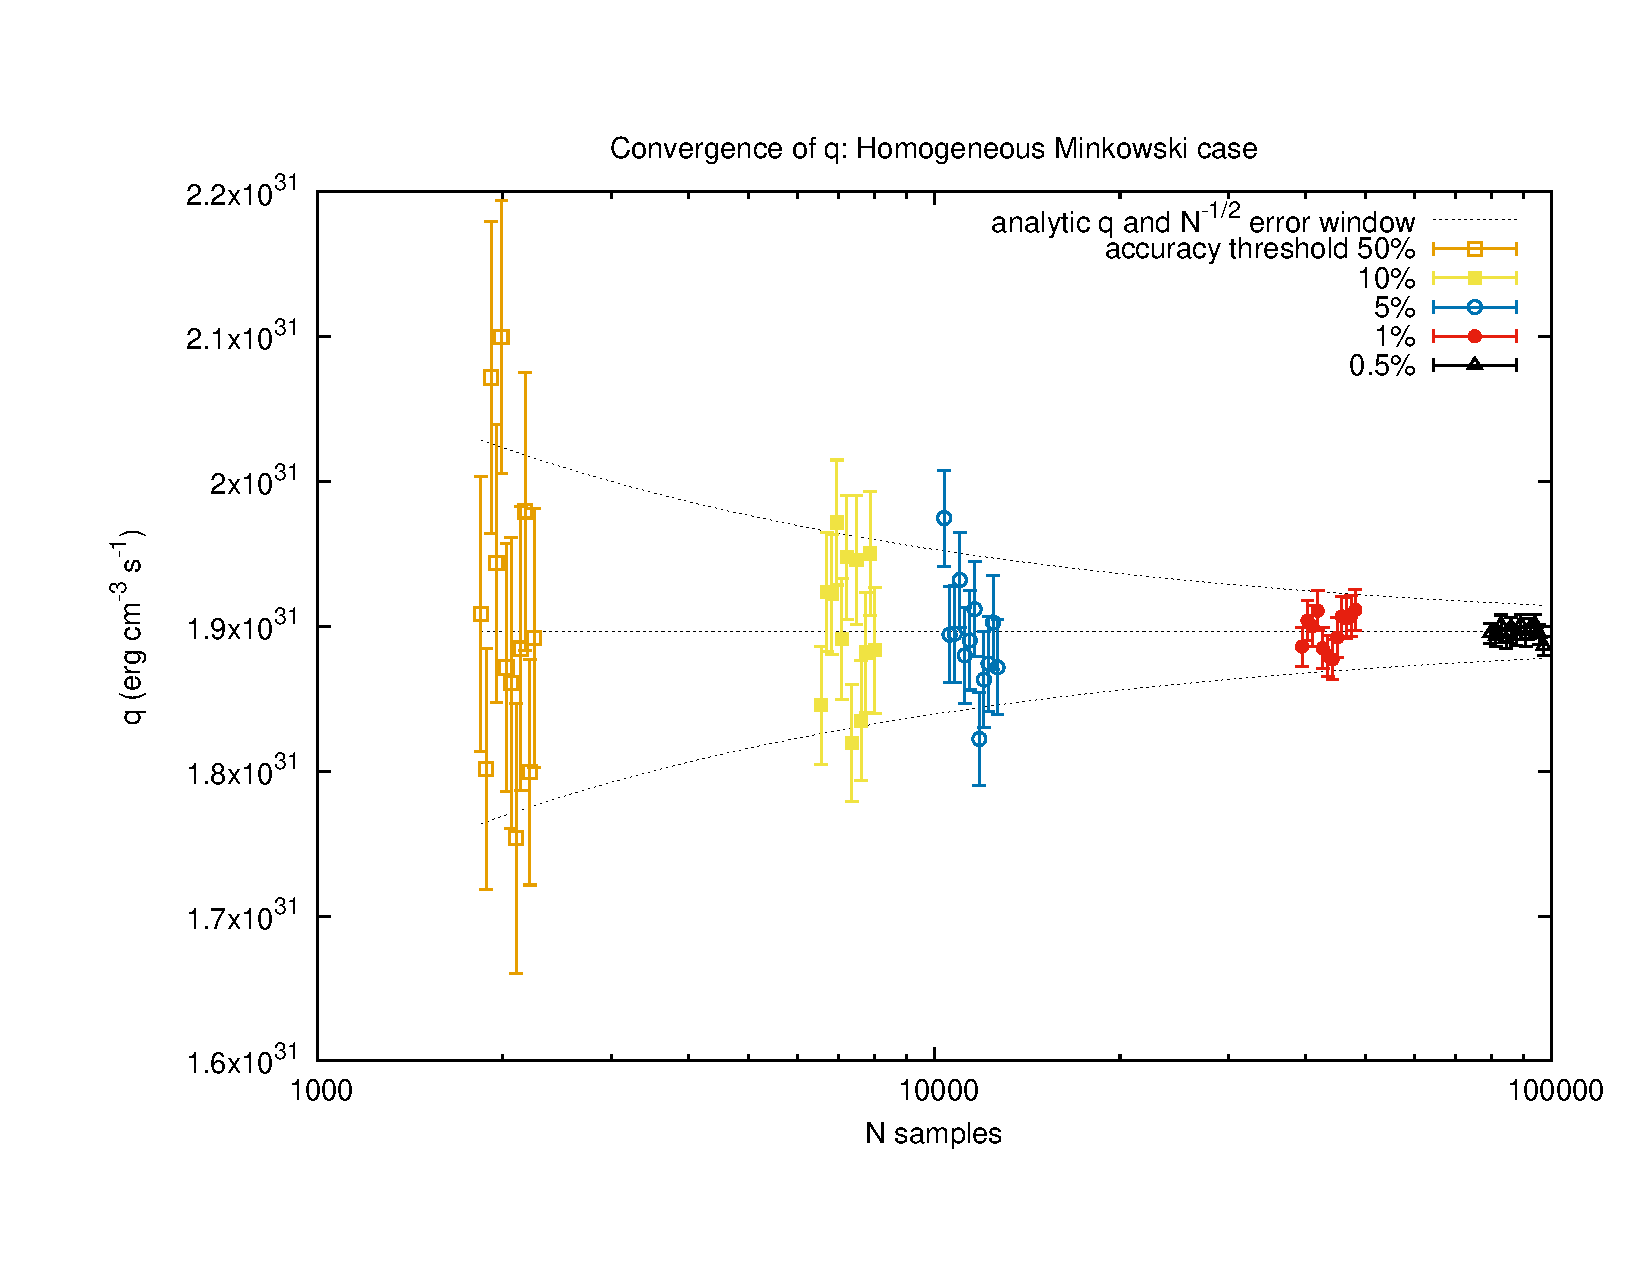
\includegraphics[width=16cm]{Figures/convergence_homogeneous_minkowski}
  \caption[Convergence of $q_{\nu\bar{\nu}}$ in the homogeneous Minkowski case]{
    Convergence of the integration estimating $q_{\nu\bar{\nu}}$ in the
    homogeneous Minkowski case.
    The horizontal axis is the number of samples of the integrand, $N$;
    the number of unique rays traced, therefore, is $2N$.
    At four different accuracy thresholds (the four clusters), I have computed
    the integral 12 times, to display the statistical scatter.
    The Vegas estimates of the error are given as as error bars.
    The legend labels each group of points by the accuracy threshold; but note,
    at low accuracy, the algorithm is bad at guessing how many samples it needs,
    so the threshold and the final error estimate disagree at low-$N$.
    The 12 points in each cluster are plotted with a small, false scatter in $N$
    to make them visually distinct.
    The dashed lines show the correct value of $q_{\nu\bar{\nu}}$ and an
    $N^{1/2}$-envelope (with an arbitrary vertical scaling to bound the points
    at the highest resolutions).
  }
  \label{fig:convergence_homo_mink}
\end{figure}

Fig.~\ref{fig:convergence_homo_mink} shows the results of a suite of
computations at increasing accuracy thresholds.
The numerical estimate of $q_{\nu\bar{\nu}}$ converges to the analytical result
faster than $N^{1/2}$ (the dotted envelope in the figure).
For an accuracy of 10\% (in this simple case) we need to compute
$\sym3\times10^3$ samples of the integrand.

\subsubsection{Hot Compact Star}
\label{sssc:q_af_sphere}
We may also analytically compute $q_{\nu\bar{\nu}}$ outside the hot compact
star presented in Sec.~\ref{sssc:f_af_sphere}.
\todo{add notes from *.nb}
In that Section, we identified a spurious
variation in $f_\nu$ across the neutrinosurface (seen in
Fig.~\ref{fig:f_hot_ns}), due to the combination of a discrete jump in opacity
at the surface, and the finite time steps used to integrate the rays
(discussed in Sec.~\ref{ssec:timestepping}).
In the integral of $q_{\nu\bar{\nu}}$ presented here, our standard settings
for the Dormand-Prince time stepping (throttling $\Delta t\leq1.5\,M_\odot$)
introduce a systematic error of 10--20\% in the integral which does not converge
away with $N$, the number of rays traced.
In order to push this systematic error in $f_\nu$ low enough to examine the
error in our Monte Carlo algorithm for $q_{\nu\bar{\nu}}$,
we have throttled the time stepping to $\Delta t \leq0.1\,M_\odot$.
At the standard timestep settings, sampling the integrand $6\times10^4$ times
takes 10~min; at this high resolution, it takes 5~hrs.

\begin{figure}
  \centering
  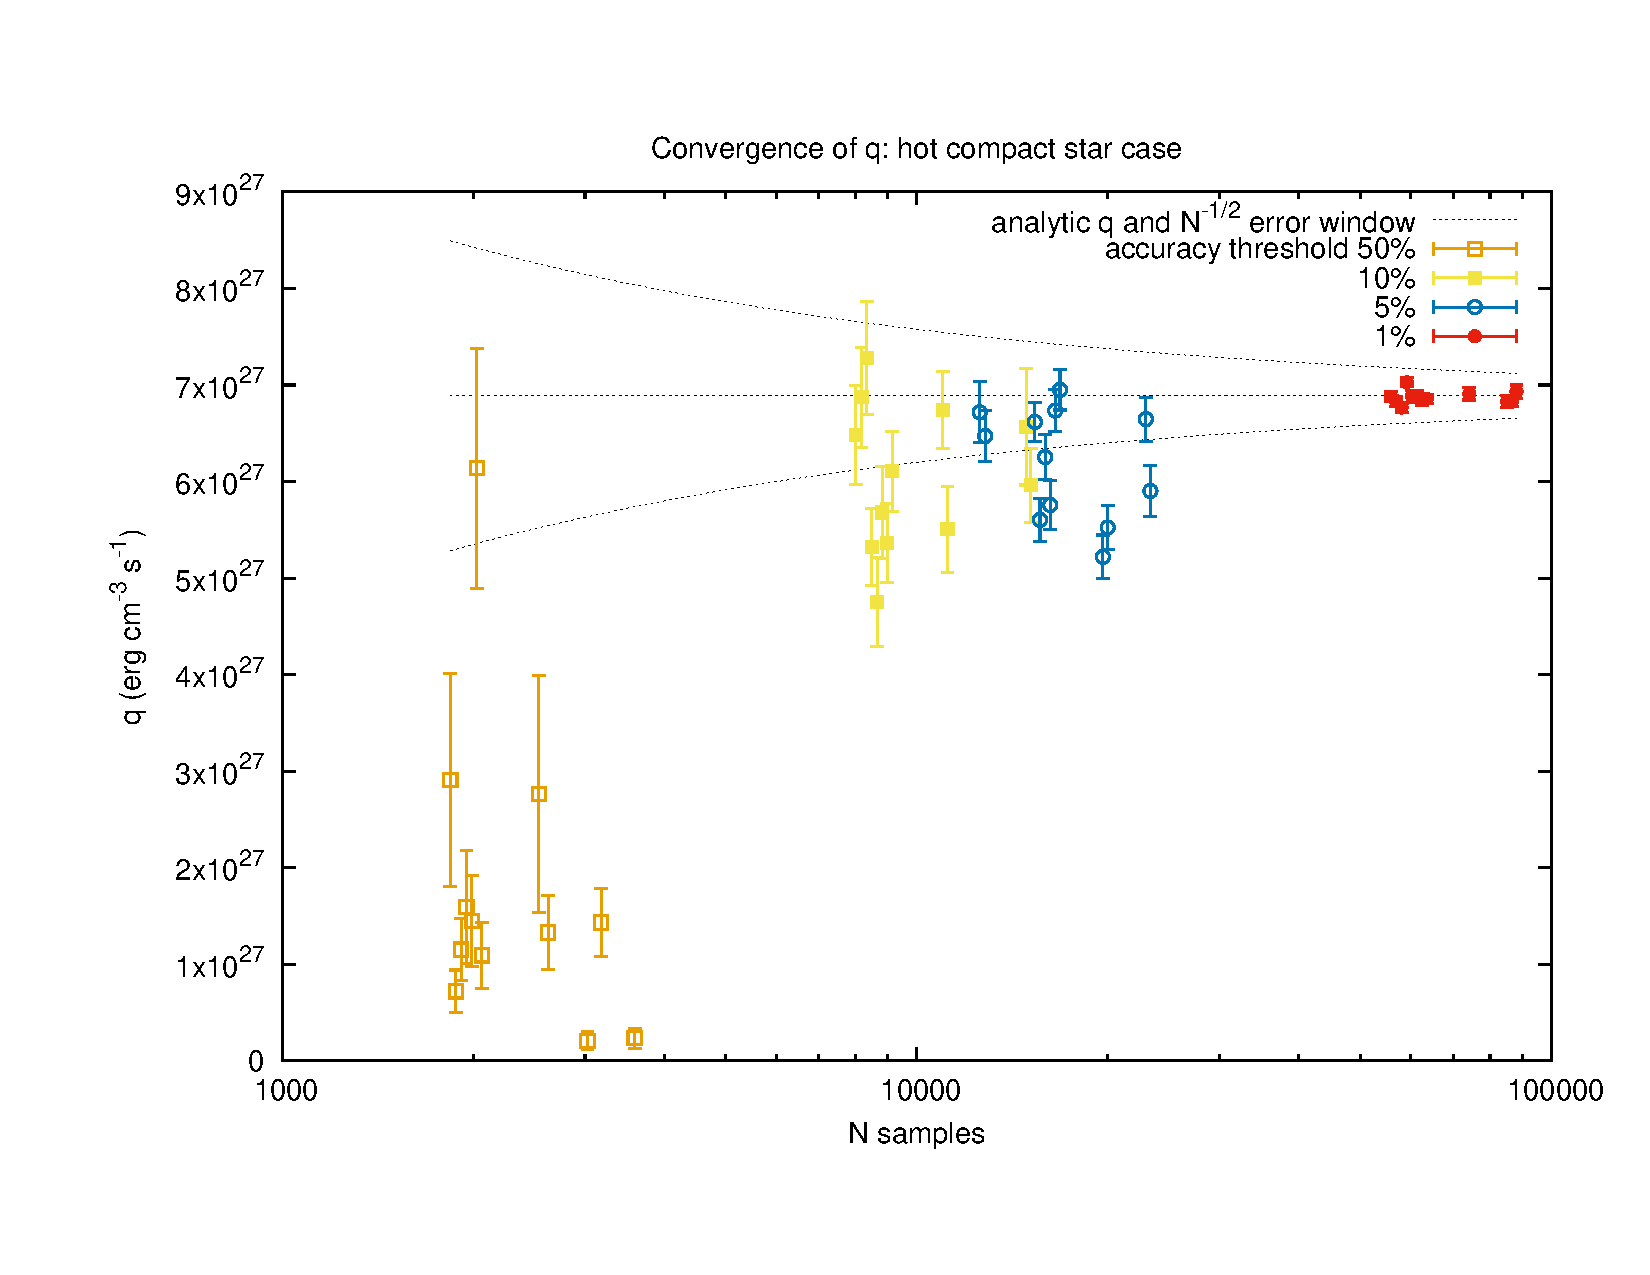
\includegraphics[width=16cm]{Figures/convergence_asano_fukuyama}
  \caption[Convergence of $q_{\nu\bar{\nu}}$ in the hot compact star case]{
    Convergence of the integration estimating $q_{\nu\bar{\nu}}$ in the
    hot compact star case.
    See caption for Fig.~\ref{fig:convergence_homo_mink} for description.
    (Note, the relative vertical range in this figure is signicantly larger
    than the range in Fig.~\ref{fig:convergence_homo_mink}.)
  }
  \label{fig:convergence_af_sphere}
\end{figure}

Fig.~\ref{fig:convergence_af_sphere} shows the results of a suite of
computations at increasing accuracy thresholds.
Unlike the homogeneous Minkowski case, here the Vegas algorithm
systematically underestimates $q_{\nu\bar{\nu}}$ at low resolutions.
For an accuracy of 10\% in this more realistic case, we need to compute
$\sym3\times10^4$ samples of the integrand.
\todo{catalog other sources for error in this case}

\section{$q_{\nu \bar{\nu}}$ for this Accretion Disk}
\label{sec:q_this_case}
We calculate $q_{\nu\bar{\nu}}$ above the accretion disk, on a unigrid, to make
an estimate of $Q_{\nu\bar{\nu}}$ (Eqn.~\ref{eqn:Q_vol}):
the power at infinite separation from the source, available to drive a jet.
In cartesian coordinates, the volume integration is decomposed
$\diff^3 x=\sqrt{-g}\, \diff x\,\diff y\,\diff z$.
\todo{add redshift factor for time}
Because of the approximate axial- and reflection-symmetry of the disk, we only
calculate $q_{\nu\bar{\nu}}$ over one octant and multiply $Q_{\nu\bar{\nu}}$ by
eight.
\todo{explain treatment of on-axis points}
The octant is shown in a meridional slice in Fig.~\ref{fig:q_grid}.
Because of the steep dependence of the annihilation rate on the relative angles
between incoming neutrino trajectories, $q_{\nu\bar{\nu}}$ falls off steeply
with distance from the bright inner region of the funnel: the rate decreases with
$r^{-8}$ at large enough distances that the source is approximately spherical
\citep{seti2006-nunubar_and_spin}.
Thus, the annihilation rate at points outside the integration grid is negligible.
In fact, the computed local annihilation rate, shown in
Fig.~\ref{fig:q_rate_meridional},
confirms that $q_{\nu\bar{\nu}}$ falls off by many orders of magnitude at the
edges of this grid.
\todo{how large $N$?}

\begin{figure}
  \centering
  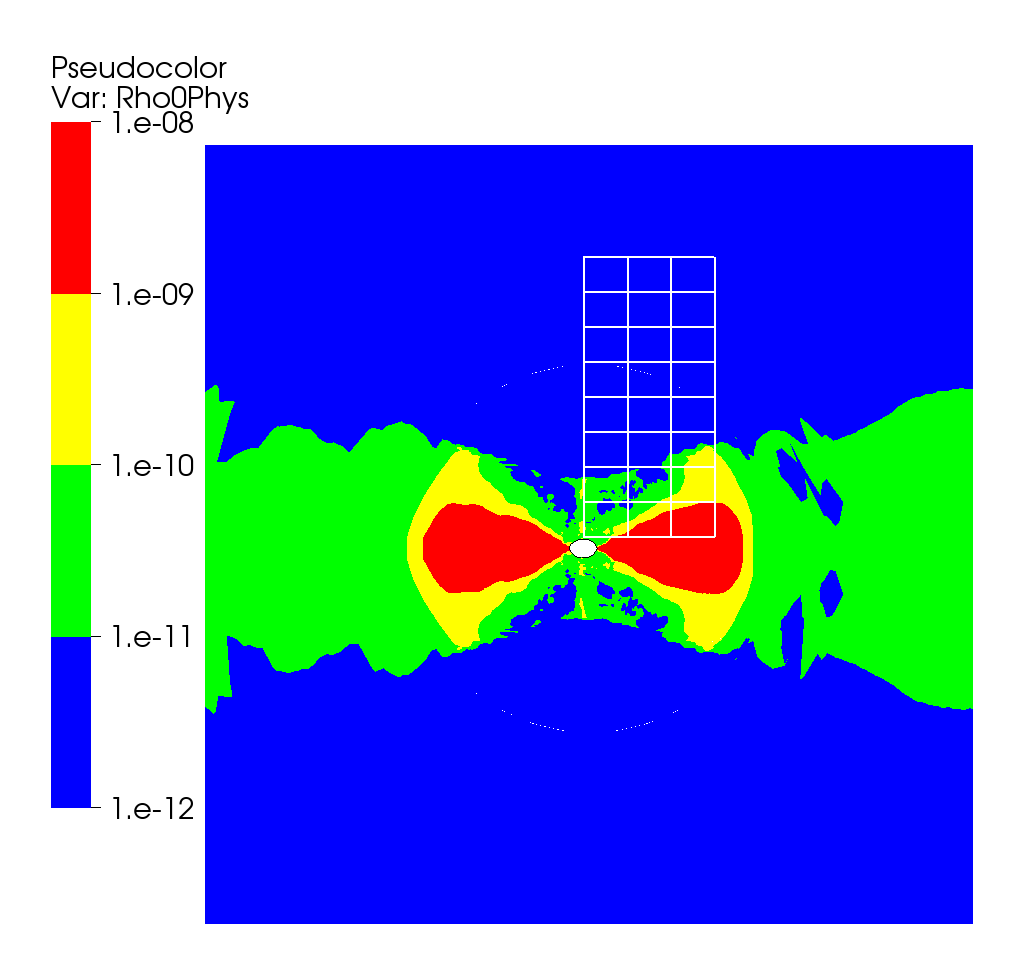
\includegraphics[width=10cm]{Figures/annihilation-slice}
  \caption[Grid used for the volume integral of $q_{\nu\bar{\nu}}$]{
    Meridional slice of the grid used to compute the spatial volume
    integral $Q_{\nu\bar{\nu}}=\int\diff^3 x\,q_{\nu\bar{\nu}}$ over one octant
    of the disk. The grid is composed of $4\times4\times9=144$~points,
    and extends 90~km, 90~km, and 192~km in the x-, y-, and z-directions,
    respectively.
    Decades of fluid rest density are plotted in units of
    $M_\odot^{-2}\sim10^{18}$~g~cm$^{-3}$.
  }
  \label{fig:q_grid}
\end{figure}

\begin{figure}
  \centering
  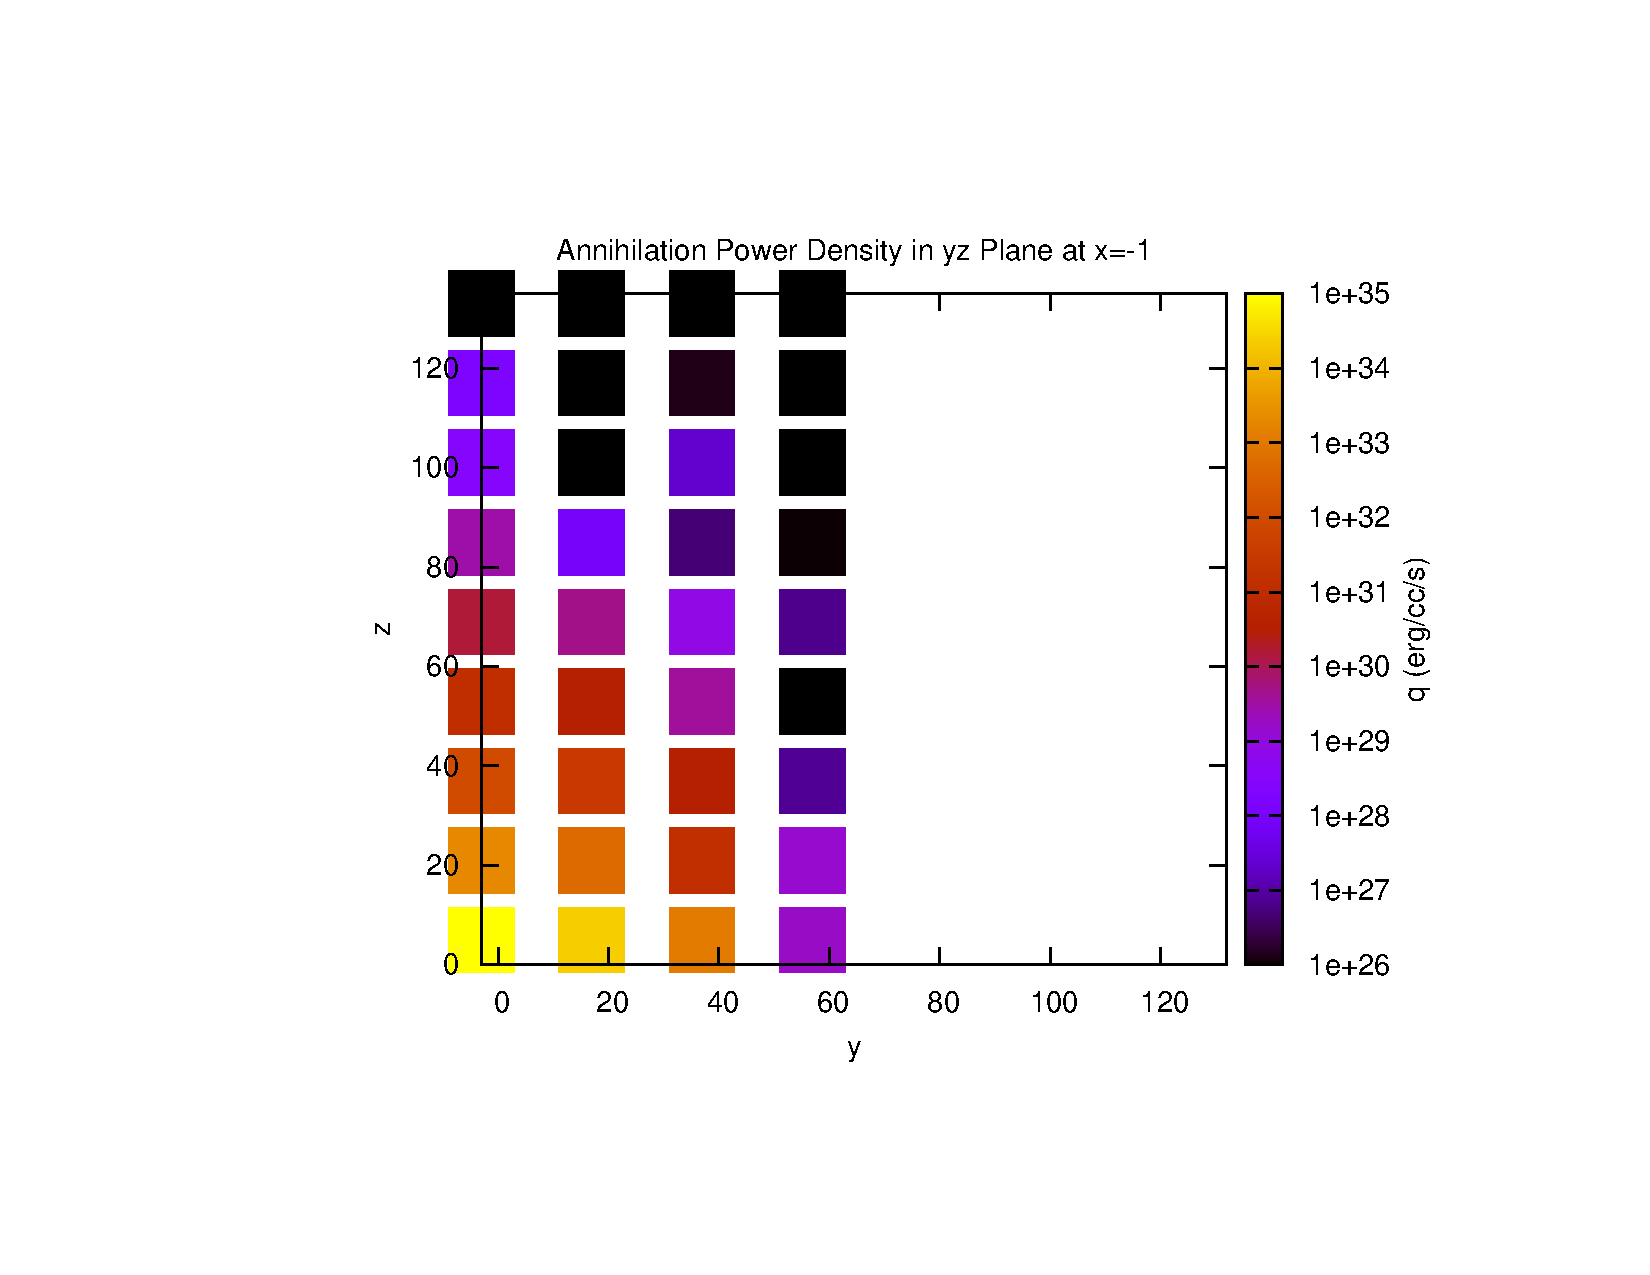
\includegraphics[width=13cm]{Figures/annihilation_rate_x-1}
  \caption[$q_{\nu\bar{\nu}}$ at the grid points]{
    Meridional slice of the annihilation rate in the y-z plane of the grid
    depicted in Fig.~\ref{fig:q_grid}. The axes are labeled in units of
    $M_\odot\sim1.5$~km.
  }
  \label{fig:q_rate_meridional}
\end{figure}

\subsection{Excluding Some Points from the Integral}
\label{ssec:excluding_pts}

The goal of our calculation is to estimate the free energy available to drive
a jet---energy carried by a superheated electron-positron pair plasma expanding
primarily away from the disk. But the simple volume integral of the points in
Fig.~\ref{fig:q_rate_meridional} includes the thermal energy of some plasma
that is headed for the black hole, and some plasma that that will be re-absorbed
by the nuclear fluid via the $\beta$-capture reactions,
$e^{-}\,p \rightarrow \nu_e\,n$ and
$e^{+}\,n \rightarrow \bar{\nu}_e\,p$.
We account for both of these losses in an approximate way by discarding points
from the volume integral at which these processes happen faster than the
explosion.

We can compare the timescales of these processes to the explosion timescale,
%which is a local estimate for how rapidly the plasma evacuates its place of
%origin, $x^j$:
%\begin{equation}
%  T_{\rm exp}(x^j) \sim \frac{q_{\nu\bar{\nu}}}{\rho}
%\end{equation}
%where $\rho$ is the rest density, which we can estimate from
%Fig.~\ref{fig:q_grid} as $\sym10^{-11}\,M_\odot^{-2}$ in the funnel region.
%\todo{untrustworthy; that's atmosphere}
which is a global estimate for how rapidly the plasma evacuates the funnel:
\begin{equation}
  T_{\rm exp} \sim \frac{L}{c_s}
\end{equation}
where $L\sim100\,M_\odot\sim0.5$~ms is the characteristic size of the funnel, and
$c_s\sim1$ is the sound speed, which is very high at these densities and
temperatures;
\todo{check $c_s$}
thus we estimate $T_{\rm exp} \sim 1$~ms.
Energy transfer processes occuring on a timescale shorter than this will quench
the explosion. We examine the processes of accretion and $\beta$-capture below.

\subsubsection{Accretion}
\label{sssc:accretion_timescale}
Very near the black hole, accretion dominates the energy transfer processes:
radiative and kinematic processes can't compete.
Energy deposited by neutrino-antineutrino annihilation in these regions
disappears into the black hole. Fig.~\ref{fig:timescales} shows the
advection timescale:
\begin{equation}
  T_{\rm adv} \sim \frac{r}{v^r}
\end{equation}
where $r$ is the radial distance from the black hole, and $v^r$ the radial
component of the fluid velocity.
Only within $r<30$~km does this process compete with the explosion.
However, this is a very rough estimate. The noise visible in the funnel region
of Fig.~\ref{fig:timescales} is due to the low densities there, where we cannot
accurately evolve the hydrodynamics equations, and where at some points,
we impose a slow-moving, low-density atmosphere, as described in
Sec.~\ref{sec:Methods}.

\begin{figure}
  \centering
  \begin{subfigure}{.45\textwidth}
    \centering
    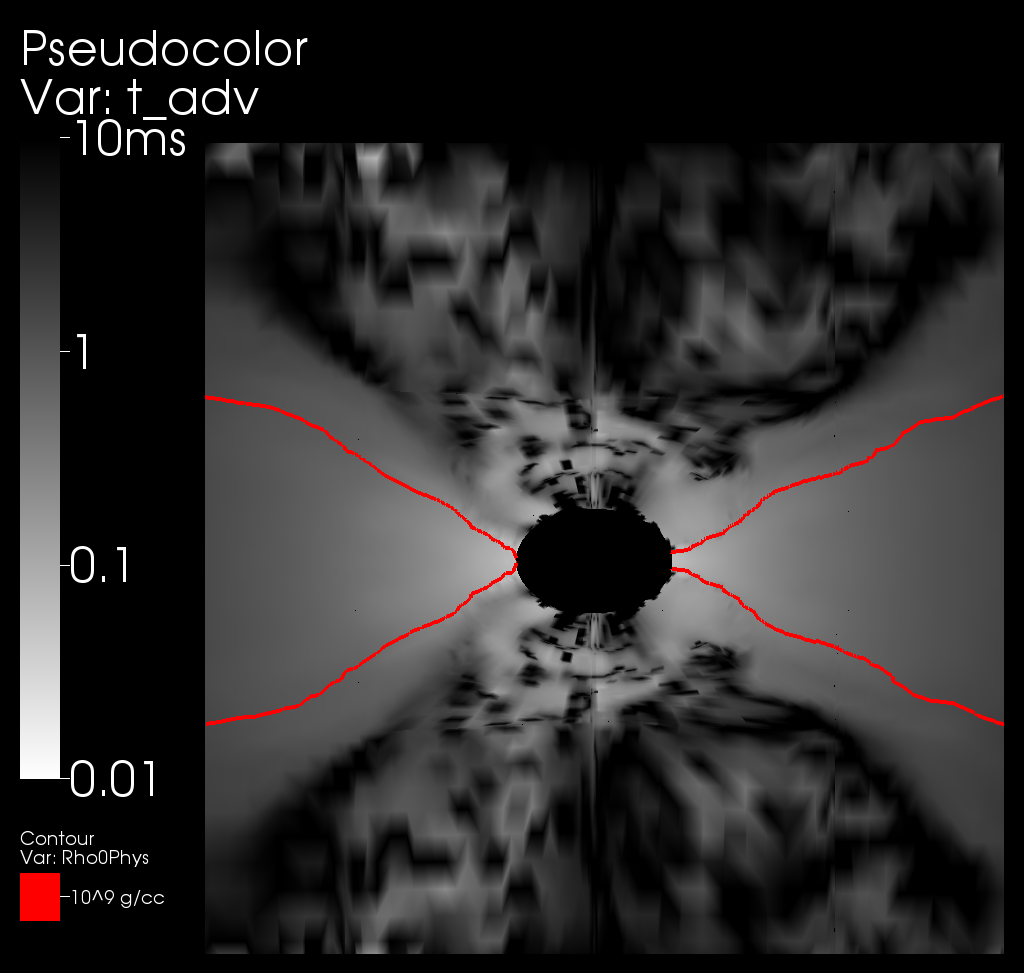
\includegraphics[width=1\linewidth]{Figures/timescales-slice-tadv}
  \end{subfigure}
  \begin{subfigure}{.45\textwidth}
    \centering
    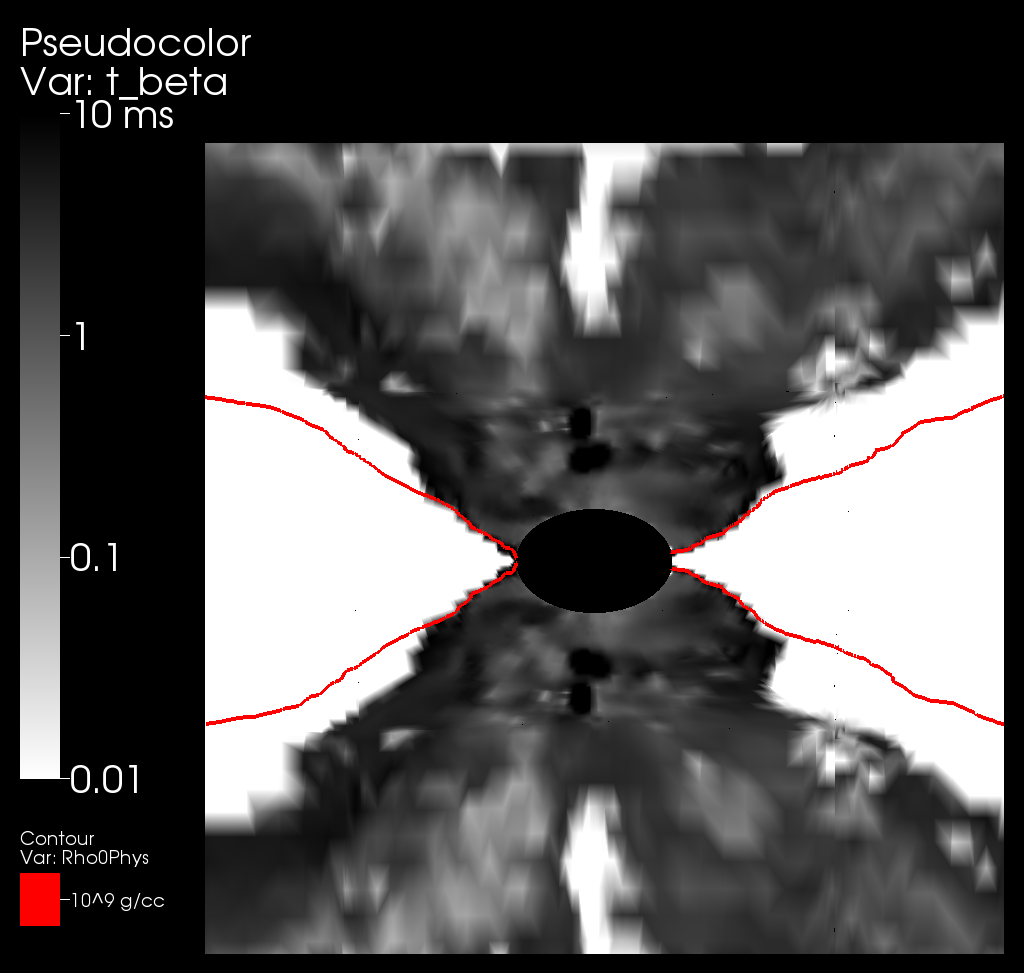
\includegraphics[width=1\linewidth]{Figures/timescales-slice-tbeta}
  \end{subfigure}
  \caption[Colormaps of explosion-quenching timescales]{
    Meridional slices of the timescales of two explosion-quenching processes,
    zoomed-in on the region $r\lesssim40$~km.
    The red density contour is drawn at $10^9\,{\rm g\,cm^{-3}}$.
    The oval in the center is the black hole horizon.
    Where $T\lesssim1$~ms, that process quenches the explosion.
    \emph{Left panel}: $T_{\rm adv}$ is noisy, and we can't really trust it in the
    funnel region, where we impose a false atmosphere at some points (described in
    Sec.~\ref{sec:Methods}).
    But I estimate that it is less than 1~ms within
    approximately three horizon-radii of the center.
    \emph{Right panel}: $T_\beta$ is clearly less than 1~ms only within the
    bulk of the disk.
  }
  \label{fig:timescales}
\end{figure}

\subsubsection{$\beta$-Capture}
\label{sssc:accretion_beta}
Deep inside the disk, the electron-positron pair plasma created by the
neutrino-antineutrino annihilation gets recaptured by nucleons, transferring
energy away from the plasma.

Fig.~\ref{fig:timescales} shows the $\beta$-capture timescale:
\begin{equation}
  T_\beta \sim \frac{n_b}{R_{\nu_e}+R_{\bar{\nu}_e}}
\end{equation}
where $n_b$ is the baryon number density, and $R_{\nu_e}$ and $R_{\bar{\nu}_e}$
are the local leakage lepton-number emission rates, a rough estimate for the
\todo{how good?}
rates of the $\beta$-capture reactions (see Sec.~\ref{sec:leakage}).
This timescale is much larger than 1~ms inside the funnel, where it may be
neglected, and much less than 1~ms inside the disk, where it quenches the
explosion.

\subsection{Back-of-the-Envelope Estimate of $Q_{\nu\bar{\nu}}$}
\label{ssec:back_of_envelope_Q}
Excluding points affected by these explosion-quenching processes, we can make an
estimate of the power at infinite separation:
\begin{equation}
  Q_{\nu\bar{\nu}} \approx 4 \pm 0.5 \times 10^{52}\, {\rm erg\,s^{-1}}\nonumber,
\end{equation}
where I have summed $q_{\nu\bar{\nu}}$ using a simple midpoint-rule
\todo{include $\pm$ order-of-mag for numer res}
\todo{add/explain redshift term}
numerical integration,
\todo{estimate midpoint err, goes as $q_{\nu\bar{\nu}}''$}
and the uncertainty is the volume integral of the uncertainties estimated by the
Monte Carlo algorithm, which we guess to be an underestimate, from the results
of the hot, compact star test in Sec.~\ref{sssc:q_af_sphere}.

To order-of-magnitude, this power is maintained for the lifetime of the disk,
$T_{\rm dep}\sim200$~ms (see Sec.~\ref{sec:scales}). Thus
\begin{equation}
  E_{\rm jet} \approx 10^{52} \, {\rm erg} \nonumber,
\end{equation}
which is comparable to the brightest luminosities and durations observed for
shoft duration gamma ray bursts:
\todo{cite Nakar 2007}
\begin{eqnarray}
  L &\sim& 10^{50\text{--}52} \, {\rm erg s^{-1}} \nonumber\\
  \langle T_{90} \rangle &\sim& 100 \,{\rm ms}. \nonumber
\end{eqnarray}
\todo{actually, $E_{\rm jet}$ is larger by factor of 10}
We conclude that in this case of a high-spin black hole and massive accretion
disk, neutrino-antineutrino annihilation is a viable candidate alone to power a
gamma ray burst.

The two serious limitations of this back-of-the-envelope calculation,
however, is 1) the error in the numerical integration over the spatial volume,
which we could improve with a Monte Carlo integration over that volume,
and 2) the numerical noise and lack of information about the state of the matter
in the funnel.
\todo{also related to lack of info about baryon loading}

